\documentclass[twoside]{book}

% Packages required by doxygen
\usepackage{fixltx2e}
\usepackage{calc}
\usepackage{doxygen}
\usepackage[export]{adjustbox} % also loads graphicx
\usepackage{graphicx}
\usepackage[utf8]{inputenc}
\usepackage{makeidx}
\usepackage{multicol}
\usepackage{multirow}
\PassOptionsToPackage{warn}{textcomp}
\usepackage{textcomp}
\usepackage[nointegrals]{wasysym}
\usepackage[table]{xcolor}

% Font selection
\usepackage[T1]{fontenc}
\usepackage[scaled=.90]{helvet}
\usepackage{courier}
\usepackage{amssymb}
\usepackage{sectsty}
\renewcommand{\familydefault}{\sfdefault}
\allsectionsfont{%
  \fontseries{bc}\selectfont%
  \color{darkgray}%
}
\renewcommand{\DoxyLabelFont}{%
  \fontseries{bc}\selectfont%
  \color{darkgray}%
}
\newcommand{\+}{\discretionary{\mbox{\scriptsize$\hookleftarrow$}}{}{}}

% Page & text layout
\usepackage{geometry}
\geometry{%
  a4paper,%
  top=2.5cm,%
  bottom=2.5cm,%
  left=2.5cm,%
  right=2.5cm%
}
\tolerance=750
\hfuzz=15pt
\hbadness=750
\setlength{\emergencystretch}{15pt}
\setlength{\parindent}{0cm}
\setlength{\parskip}{3ex plus 2ex minus 2ex}
\makeatletter
\renewcommand{\paragraph}{%
  \@startsection{paragraph}{4}{0ex}{-1.0ex}{1.0ex}{%
    \normalfont\normalsize\bfseries\SS@parafont%
  }%
}
\renewcommand{\subparagraph}{%
  \@startsection{subparagraph}{5}{0ex}{-1.0ex}{1.0ex}{%
    \normalfont\normalsize\bfseries\SS@subparafont%
  }%
}
\makeatother

% Headers & footers
\usepackage{fancyhdr}
\pagestyle{fancyplain}
\fancyhead[LE]{\fancyplain{}{\bfseries\thepage}}
\fancyhead[CE]{\fancyplain{}{}}
\fancyhead[RE]{\fancyplain{}{\bfseries\leftmark}}
\fancyhead[LO]{\fancyplain{}{\bfseries\rightmark}}
\fancyhead[CO]{\fancyplain{}{}}
\fancyhead[RO]{\fancyplain{}{\bfseries\thepage}}
\fancyfoot[LE]{\fancyplain{}{}}
\fancyfoot[CE]{\fancyplain{}{}}
\fancyfoot[RE]{\fancyplain{}{\bfseries\scriptsize Generated by Doxygen }}
\fancyfoot[LO]{\fancyplain{}{\bfseries\scriptsize Generated by Doxygen }}
\fancyfoot[CO]{\fancyplain{}{}}
\fancyfoot[RO]{\fancyplain{}{}}
\renewcommand{\footrulewidth}{0.4pt}
\renewcommand{\chaptermark}[1]{%
  \markboth{#1}{}%
}
\renewcommand{\sectionmark}[1]{%
  \markright{\thesection\ #1}%
}

% Indices & bibliography
\usepackage{natbib}
\usepackage[titles]{tocloft}
\setcounter{tocdepth}{3}
\setcounter{secnumdepth}{5}
\makeindex

% Hyperlinks (required, but should be loaded last)
\usepackage{ifpdf}
\ifpdf
  \usepackage[pdftex,pagebackref=true]{hyperref}
\else
  \usepackage[ps2pdf,pagebackref=true]{hyperref}
\fi
\hypersetup{%
  colorlinks=true,%
  linkcolor=blue,%
  citecolor=blue,%
  unicode%
}

% Custom commands
\newcommand{\clearemptydoublepage}{%
  \newpage{\pagestyle{empty}\cleardoublepage}%
}

\usepackage{caption}
\captionsetup{labelsep=space,justification=centering,font={bf},singlelinecheck=off,skip=4pt,position=top}

%===== C O N T E N T S =====

\begin{document}

% Titlepage & ToC
\hypersetup{pageanchor=false,
             bookmarksnumbered=true,
             pdfencoding=unicode
            }
\pagenumbering{alph}
\begin{titlepage}
\vspace*{7cm}
\begin{center}%
{\Large My Project }\\
\vspace*{1cm}
{\large Generated by Doxygen 1.8.14}\\
\end{center}
\end{titlepage}
\clearemptydoublepage
\pagenumbering{roman}
\tableofcontents
\clearemptydoublepage
\pagenumbering{arabic}
\hypersetup{pageanchor=true}

%--- Begin generated contents ---
\chapter{Bio\+Net}
\label{md__r_e_a_d_m_e}
\Hypertarget{md__r_e_a_d_m_e}
A generic network class for biology. 
\chapter{Hierarchical Index}
\section{Class Hierarchy}
This inheritance list is sorted roughly, but not completely, alphabetically\+:\begin{DoxyCompactList}
\item \contentsline{section}{Adj}{\pageref{class_adj}}{}
\begin{DoxyCompactList}
\item \contentsline{section}{Bio\+Adj$<$ T $>$}{\pageref{class_bio_adj}}{}
\begin{DoxyCompactList}
\item \contentsline{section}{Bio\+Adj\+List$<$ T $>$}{\pageref{class_bio_adj_list}}{}
\item \contentsline{section}{Bio\+Adj\+Mat$<$ T $>$}{\pageref{class_bio_adj_mat}}{}
\end{DoxyCompactList}
\end{DoxyCompactList}
\item \contentsline{section}{Bio\+Edge$<$ T $>$}{\pageref{class_bio_edge}}{}
\item \contentsline{section}{Bio\+List$<$ T $>$}{\pageref{class_bio_list}}{}
\item \contentsline{section}{Bio\+Net$<$ T $>$}{\pageref{class_bio_net}}{}
\item \contentsline{section}{C\+S\+V\+Reader}{\pageref{class_c_s_v_reader}}{}
\item \contentsline{section}{Edge}{\pageref{struct_edge}}{}
\item exception\begin{DoxyCompactList}
\item \contentsline{section}{Bio\+Net\+Exception}{\pageref{class_bio_net_exception}}{}
\begin{DoxyCompactList}
\item \contentsline{section}{Data\+Invalid\+Format\+Exception}{\pageref{class_data_invalid_format_exception}}{}
\item \contentsline{section}{File\+Not\+Exist\+Exception}{\pageref{class_file_not_exist_exception}}{}
\item \contentsline{section}{Incorrect\+File\+Format\+Exception}{\pageref{class_incorrect_file_format_exception}}{}
\end{DoxyCompactList}
\end{DoxyCompactList}
\item \contentsline{section}{File\+Handler}{\pageref{class_file_handler}}{}
\begin{DoxyCompactList}
\item \contentsline{section}{G\+M\+L\+Handler}{\pageref{class_g_m_l_handler}}{}
\end{DoxyCompactList}
\item \contentsline{section}{IO}{\pageref{class_i_o}}{}
\begin{DoxyCompactList}
\item \contentsline{section}{Reader}{\pageref{class_reader}}{}
\begin{DoxyCompactList}
\item \contentsline{section}{Read\+Writer}{\pageref{class_read_writer}}{}
\end{DoxyCompactList}
\item \contentsline{section}{Writer}{\pageref{class_writer}}{}
\begin{DoxyCompactList}
\item \contentsline{section}{Read\+Writer}{\pageref{class_read_writer}}{}
\end{DoxyCompactList}
\end{DoxyCompactList}
\item \contentsline{section}{Node}{\pageref{struct_node}}{}
\item \contentsline{section}{Register}{\pageref{struct_register}}{}
\end{DoxyCompactList}

\chapter{Class Index}
\section{Class List}
Here are the classes, structs, unions and interfaces with brief descriptions\+:\begin{DoxyCompactList}
\item\contentsline{section}{\hyperlink{class_adj}{Adj} }{\pageref{class_adj}}{}
\item\contentsline{section}{\hyperlink{class_bio_adj}{Bio\+Adj$<$ T $>$} }{\pageref{class_bio_adj}}{}
\item\contentsline{section}{\hyperlink{class_bio_adj_list}{Bio\+Adj\+List$<$ T $>$} }{\pageref{class_bio_adj_list}}{}
\item\contentsline{section}{\hyperlink{class_bio_adj_mat}{Bio\+Adj\+Mat$<$ T $>$} }{\pageref{class_bio_adj_mat}}{}
\item\contentsline{section}{\hyperlink{class_bio_edge}{Bio\+Edge$<$ T $>$} }{\pageref{class_bio_edge}}{}
\item\contentsline{section}{\hyperlink{class_bio_list}{Bio\+List$<$ T $>$} }{\pageref{class_bio_list}}{}
\item\contentsline{section}{\hyperlink{class_bio_net}{Bio\+Net$<$ T $>$} }{\pageref{class_bio_net}}{}
\item\contentsline{section}{\hyperlink{class_bio_net_exception}{Bio\+Net\+Exception} }{\pageref{class_bio_net_exception}}{}
\item\contentsline{section}{\hyperlink{class_c_s_v_reader}{C\+S\+V\+Reader} }{\pageref{class_c_s_v_reader}}{}
\item\contentsline{section}{\hyperlink{class_data_invalid_format_exception}{Data\+Invalid\+Format\+Exception} }{\pageref{class_data_invalid_format_exception}}{}
\item\contentsline{section}{\hyperlink{struct_edge}{Edge} }{\pageref{struct_edge}}{}
\item\contentsline{section}{\hyperlink{class_file_handler}{File\+Handler} }{\pageref{class_file_handler}}{}
\item\contentsline{section}{\hyperlink{class_file_not_exist_exception}{File\+Not\+Exist\+Exception} }{\pageref{class_file_not_exist_exception}}{}
\item\contentsline{section}{\hyperlink{class_g_m_l_handler}{G\+M\+L\+Handler} }{\pageref{class_g_m_l_handler}}{}
\item\contentsline{section}{\hyperlink{class_incorrect_file_format_exception}{Incorrect\+File\+Format\+Exception} }{\pageref{class_incorrect_file_format_exception}}{}
\item\contentsline{section}{\hyperlink{class_i_o}{IO} }{\pageref{class_i_o}}{}
\item\contentsline{section}{\hyperlink{struct_node}{Node} }{\pageref{struct_node}}{}
\item\contentsline{section}{\hyperlink{class_reader}{Reader} }{\pageref{class_reader}}{}
\item\contentsline{section}{\hyperlink{class_read_writer}{Read\+Writer} }{\pageref{class_read_writer}}{}
\item\contentsline{section}{\hyperlink{struct_register}{Register} }{\pageref{struct_register}}{}
\item\contentsline{section}{\hyperlink{class_writer}{Writer} }{\pageref{class_writer}}{}
\end{DoxyCompactList}

\chapter{Class Documentation}
\hypertarget{class_adj}{}\section{Adj Class Reference}
\label{class_adj}\index{Adj@{Adj}}
Inheritance diagram for Adj\+:\begin{figure}[H]
\begin{center}
\leavevmode
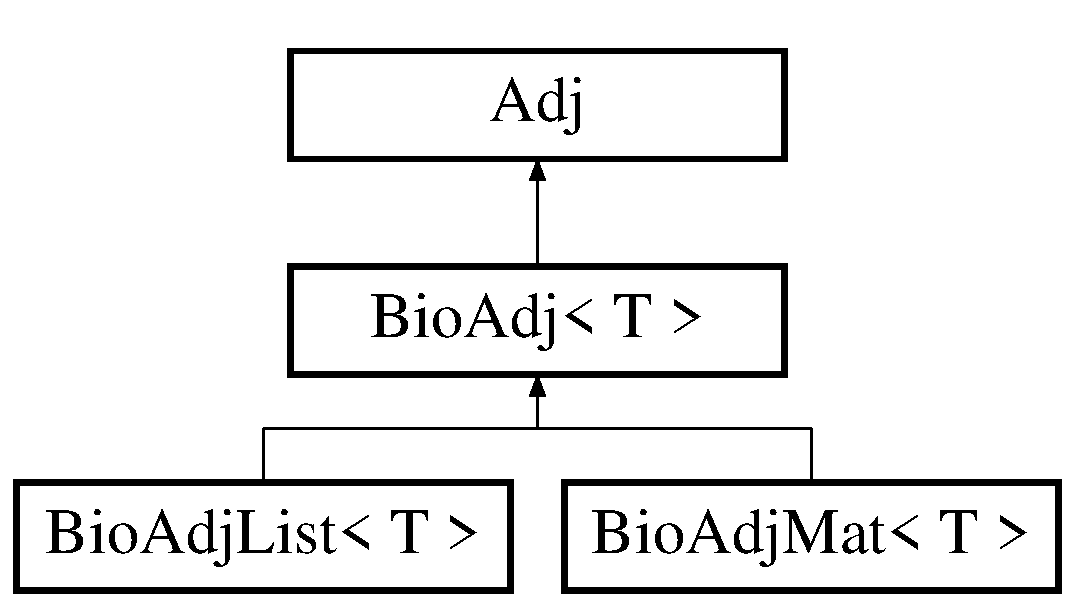
\includegraphics[height=3.000000cm]{class_adj}
\end{center}
\end{figure}


The documentation for this class was generated from the following file\+:\begin{DoxyCompactItemize}
\item 
Bio\+Adj.\+h\end{DoxyCompactItemize}

\hypertarget{class_bio_adj}{}\section{Bio\+Adj$<$ T $>$ Class Template Reference}
\label{class_bio_adj}\index{Bio\+Adj$<$ T $>$@{Bio\+Adj$<$ T $>$}}
Inheritance diagram for Bio\+Adj$<$ T $>$\+:\begin{figure}[H]
\begin{center}
\leavevmode
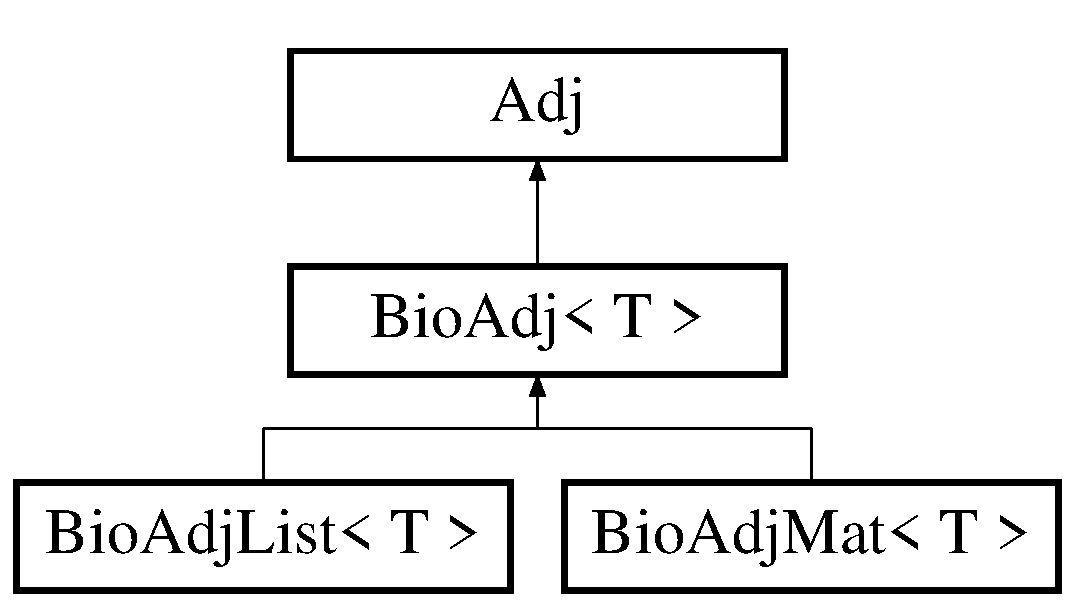
\includegraphics[height=3.000000cm]{class_bio_adj}
\end{center}
\end{figure}
\subsection*{Public Member Functions}
\begin{DoxyCompactItemize}
\item 
\mbox{\Hypertarget{class_bio_adj_aa769d5822736685bff5387839fb3a718}\label{class_bio_adj_aa769d5822736685bff5387839fb3a718}} 
virtual void {\bfseries set\+Edge} (const int, const int, const T)=0
\item 
\mbox{\Hypertarget{class_bio_adj_a1446c65a9d7c858dea0666a055319dbc}\label{class_bio_adj_a1446c65a9d7c858dea0666a055319dbc}} 
virtual void {\bfseries set\+Edge} (const string \&, const string \&, const T)=0
\item 
\mbox{\Hypertarget{class_bio_adj_a3958a7fb058da16d1bf99917aae4f227}\label{class_bio_adj_a3958a7fb058da16d1bf99917aae4f227}} 
virtual T {\bfseries get\+Edge} (const int, const int) const =0
\item 
\mbox{\Hypertarget{class_bio_adj_a625584cda56942b795cfb5aa7ff63b42}\label{class_bio_adj_a625584cda56942b795cfb5aa7ff63b42}} 
virtual T {\bfseries get\+Edge} (const string \&, const string \&) const =0
\item 
\mbox{\Hypertarget{class_bio_adj_adcb60a6cbe5e02272d539a8f6acbcbce}\label{class_bio_adj_adcb60a6cbe5e02272d539a8f6acbcbce}} 
virtual void {\bfseries set\+Node} (const int, const string \&)=0
\item 
\mbox{\Hypertarget{class_bio_adj_a41a61bc0441f47afa830b0176334b4af}\label{class_bio_adj_a41a61bc0441f47afa830b0176334b4af}} 
virtual string {\bfseries get\+Node} (const int) const =0
\item 
\mbox{\Hypertarget{class_bio_adj_a19e961d134078fa680125903209bb892}\label{class_bio_adj_a19e961d134078fa680125903209bb892}} 
virtual int {\bfseries size} () const =0
\item 
\mbox{\Hypertarget{class_bio_adj_af67b3d3c3adbc270dce5e67d8c417b44}\label{class_bio_adj_af67b3d3c3adbc270dce5e67d8c417b44}} 
virtual T {\bfseries degree} (const int) const =0
\item 
\mbox{\Hypertarget{class_bio_adj_a25be2b0097f458266fdd6ee60c5c5bc0}\label{class_bio_adj_a25be2b0097f458266fdd6ee60c5c5bc0}} 
virtual int {\bfseries number\+Of\+Edges} () const =0
\item 
\mbox{\Hypertarget{class_bio_adj_a8599f66bb28493d6476bfc812b1956d4}\label{class_bio_adj_a8599f66bb28493d6476bfc812b1956d4}} 
virtual void {\bfseries resize} (const int)=0
\item 
\mbox{\Hypertarget{class_bio_adj_ab6a4252e06dcd04ab5fc3fd93765dff2}\label{class_bio_adj_ab6a4252e06dcd04ab5fc3fd93765dff2}} 
virtual int {\bfseries find\+Node\+Index} (const string \&) const =0
\item 
\mbox{\Hypertarget{class_bio_adj_ab80a3d3792670fdf6afbee2efe449433}\label{class_bio_adj_ab80a3d3792670fdf6afbee2efe449433}} 
virtual void {\bfseries delete\+Edge} (const string \&, const string \&)=0
\item 
\mbox{\Hypertarget{class_bio_adj_aab6e36e1bc6de746f7714a1627b2074d}\label{class_bio_adj_aab6e36e1bc6de746f7714a1627b2074d}} 
virtual void {\bfseries delete\+Edge} (int, int)=0
\item 
\mbox{\Hypertarget{class_bio_adj_a549d96f7306ac6a74f4ec10423a2da95}\label{class_bio_adj_a549d96f7306ac6a74f4ec10423a2da95}} 
virtual void {\bfseries delete\+Node} (const string \&)=0
\item 
\mbox{\Hypertarget{class_bio_adj_a1d620a89793f3f4af60e07fbf848c7b1}\label{class_bio_adj_a1d620a89793f3f4af60e07fbf848c7b1}} 
virtual void {\bfseries delete\+Node} (int)=0
\item 
\mbox{\Hypertarget{class_bio_adj_a24737d6b6867062e03cedd1dcccdeaa6}\label{class_bio_adj_a24737d6b6867062e03cedd1dcccdeaa6}} 
virtual void {\bfseries add\+Node} (const string \&)=0
\item 
\mbox{\Hypertarget{class_bio_adj_af7ec8cf68fa80bfe192ddee065a00b22}\label{class_bio_adj_af7ec8cf68fa80bfe192ddee065a00b22}} 
virtual void {\bfseries copy} (const \hyperlink{class_bio_adj}{Bio\+Adj}$<$ T $>$ $\ast$rhs)=0
\item 
\mbox{\Hypertarget{class_bio_adj_a6553d8cf9317f0f6553e626839cc41e9}\label{class_bio_adj_a6553d8cf9317f0f6553e626839cc41e9}} 
virtual bool {\bfseries is\+Equal} (const \hyperlink{class_bio_adj}{Bio\+Adj}$<$ T $>$ $\ast$)=0
\item 
\mbox{\Hypertarget{class_bio_adj_acebd2c08806e7c42fe9b58dcaf7fdc29}\label{class_bio_adj_acebd2c08806e7c42fe9b58dcaf7fdc29}} 
virtual void {\bfseries scale\+Up} (const T)=0
\item 
\mbox{\Hypertarget{class_bio_adj_a9fa6051fb10352bd89f0dab29787dff6}\label{class_bio_adj_a9fa6051fb10352bd89f0dab29787dff6}} 
virtual void {\bfseries scale\+Down} (const T)=0
\item 
\mbox{\Hypertarget{class_bio_adj_af1e70e3ea88acd3de861d60ad9997ff0}\label{class_bio_adj_af1e70e3ea88acd3de861d60ad9997ff0}} 
const auto \& {\bfseries get\+Keyword} ()
\item 
\mbox{\Hypertarget{class_bio_adj_aa5e3374c3c4e26f2d0339baadeba29a4}\label{class_bio_adj_aa5e3374c3c4e26f2d0339baadeba29a4}} 
{\footnotesize template$<$typename U $>$ }\\void {\bfseries copy} (const \hyperlink{class_bio_adj}{Bio\+Adj}$<$ U $>$ $\ast$rhs)
\item 
\mbox{\Hypertarget{class_bio_adj_ad36832230f726734c44b78935994e33c}\label{class_bio_adj_ad36832230f726734c44b78935994e33c}} 
{\footnotesize template$<$typename U $>$ }\\bool {\bfseries is\+Equal} (const \hyperlink{class_bio_adj}{Bio\+Adj}$<$ U $>$ $\ast$rhs)
\end{DoxyCompactItemize}
\subsection*{Protected Attributes}
\begin{DoxyCompactItemize}
\item 
\mbox{\Hypertarget{class_bio_adj_ae86137508fe8e374f845c85b0c796d76}\label{class_bio_adj_ae86137508fe8e374f845c85b0c796d76}} 
string {\bfseries keyword}
\end{DoxyCompactItemize}


The documentation for this class was generated from the following file\+:\begin{DoxyCompactItemize}
\item 
Bio\+Adj.\+h\end{DoxyCompactItemize}

\hypertarget{class_bio_adj_list}{}\section{Bio\+Adj\+List$<$ T $>$ Class Template Reference}
\label{class_bio_adj_list}\index{Bio\+Adj\+List$<$ T $>$@{Bio\+Adj\+List$<$ T $>$}}
Inheritance diagram for Bio\+Adj\+List$<$ T $>$\+:\begin{figure}[H]
\begin{center}
\leavevmode
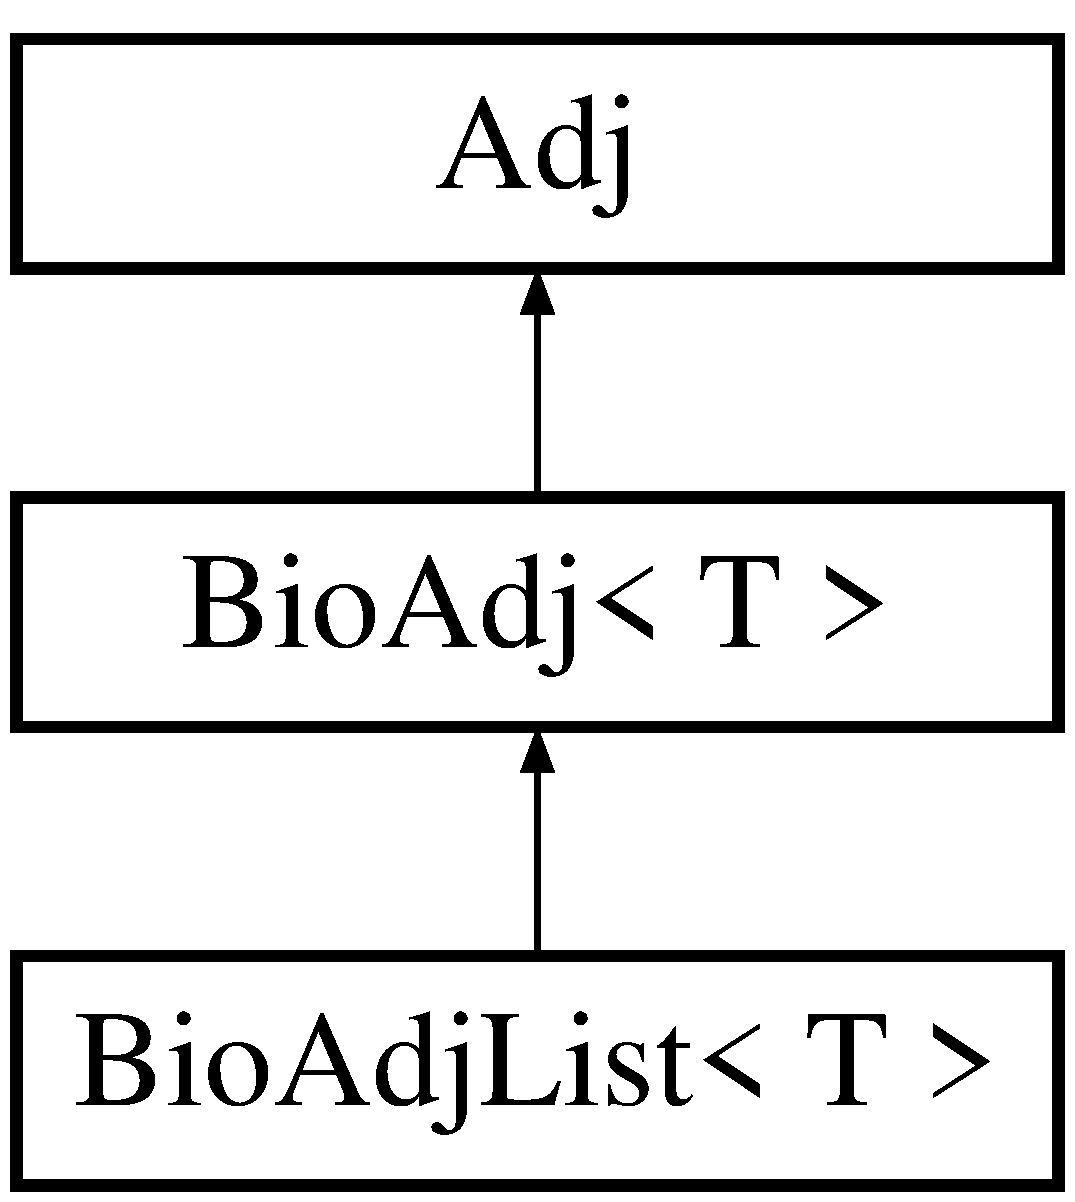
\includegraphics[height=3.000000cm]{class_bio_adj_list}
\end{center}
\end{figure}
\subsection*{Public Member Functions}
\begin{DoxyCompactItemize}
\item 
\mbox{\Hypertarget{class_bio_adj_list_a4597c403282b4db42c5ca993b9bb764a}\label{class_bio_adj_list_a4597c403282b4db42c5ca993b9bb764a}} 
{\bfseries Bio\+Adj\+List} (const \hyperlink{class_bio_adj_list}{Bio\+Adj\+List} \&copy)
\item 
\mbox{\Hypertarget{class_bio_adj_list_ad2a8808b11b3dc17553b401ff237dff4}\label{class_bio_adj_list_ad2a8808b11b3dc17553b401ff237dff4}} 
{\bfseries Bio\+Adj\+List} (int i=5)
\item 
\mbox{\Hypertarget{class_bio_adj_list_a8580717d24e223802bf52c1494691ead}\label{class_bio_adj_list_a8580717d24e223802bf52c1494691ead}} 
void {\bfseries set\+Edge} (const int x, const int y, const T w)
\item 
\mbox{\Hypertarget{class_bio_adj_list_a7e8398ed791acacc9c529a87596e9bef}\label{class_bio_adj_list_a7e8398ed791acacc9c529a87596e9bef}} 
void {\bfseries set\+Edge} (const string \&x, const string \&y, const T w)
\item 
\mbox{\Hypertarget{class_bio_adj_list_a3f19ee385ef649b18b587e97b32374fe}\label{class_bio_adj_list_a3f19ee385ef649b18b587e97b32374fe}} 
T {\bfseries get\+Edge} (const int x, const int y) const
\item 
\mbox{\Hypertarget{class_bio_adj_list_a79e53adb701489a96d2947ac36c91e75}\label{class_bio_adj_list_a79e53adb701489a96d2947ac36c91e75}} 
T {\bfseries get\+Edge} (const string \&a, const string \&b) const
\item 
\mbox{\Hypertarget{class_bio_adj_list_a2128839ac64905df63cc12eac500cbe2}\label{class_bio_adj_list_a2128839ac64905df63cc12eac500cbe2}} 
void {\bfseries set\+Node} (const int i, const string \&s)
\item 
\mbox{\Hypertarget{class_bio_adj_list_a7b1778b7290eb0b9b0e9184e494d2d47}\label{class_bio_adj_list_a7b1778b7290eb0b9b0e9184e494d2d47}} 
string {\bfseries get\+Node} (const int i) const
\item 
\mbox{\Hypertarget{class_bio_adj_list_ae5adb02ab6f4c17904f5f828b23600e5}\label{class_bio_adj_list_ae5adb02ab6f4c17904f5f828b23600e5}} 
int {\bfseries size} () const
\item 
\mbox{\Hypertarget{class_bio_adj_list_a4f7848dee4733e33afde1b31092952cd}\label{class_bio_adj_list_a4f7848dee4733e33afde1b31092952cd}} 
T {\bfseries degree} (const int x) const
\item 
\mbox{\Hypertarget{class_bio_adj_list_a2f70bb3a138c17bb8bb7cf02e6dd12f4}\label{class_bio_adj_list_a2f70bb3a138c17bb8bb7cf02e6dd12f4}} 
int {\bfseries number\+Of\+Edges} () const
\item 
\mbox{\Hypertarget{class_bio_adj_list_ac55fcd3f183f786e8352f1f81cfb0056}\label{class_bio_adj_list_ac55fcd3f183f786e8352f1f81cfb0056}} 
void {\bfseries resize} (const int new\+Size)
\item 
\mbox{\Hypertarget{class_bio_adj_list_a37b6c5c788259af6307a59ba0badb985}\label{class_bio_adj_list_a37b6c5c788259af6307a59ba0badb985}} 
int {\bfseries find\+Node\+Index} (const string \&name) const
\item 
\mbox{\Hypertarget{class_bio_adj_list_a55eb65879271ca6722ba19af93a4fd8c}\label{class_bio_adj_list_a55eb65879271ca6722ba19af93a4fd8c}} 
void {\bfseries delete\+Edge} (const string \&x, const string \&y)
\item 
\mbox{\Hypertarget{class_bio_adj_list_aa2b060c216162352ac58ec2eddead199}\label{class_bio_adj_list_aa2b060c216162352ac58ec2eddead199}} 
void {\bfseries delete\+Edge} (int x, int y)
\item 
\mbox{\Hypertarget{class_bio_adj_list_a9e2bc76c559cf676565e930b3f57433a}\label{class_bio_adj_list_a9e2bc76c559cf676565e930b3f57433a}} 
void {\bfseries delete\+Node} (const string \&name)
\item 
\mbox{\Hypertarget{class_bio_adj_list_a1d22ffb38372caa9922e458f0c587c63}\label{class_bio_adj_list_a1d22ffb38372caa9922e458f0c587c63}} 
void {\bfseries delete\+Node} (int index)
\item 
\mbox{\Hypertarget{class_bio_adj_list_a5a0d3d456727ffc1728ef6ef1f3356bd}\label{class_bio_adj_list_a5a0d3d456727ffc1728ef6ef1f3356bd}} 
void {\bfseries copy} (const \hyperlink{class_bio_adj}{Bio\+Adj}$<$ T $>$ $\ast$rhs)
\item 
\mbox{\Hypertarget{class_bio_adj_list_ac0508b6a85df7fb7965b7e80e1b6a36a}\label{class_bio_adj_list_ac0508b6a85df7fb7965b7e80e1b6a36a}} 
void {\bfseries scale\+Weights} (const T \&scale)
\item 
\mbox{\Hypertarget{class_bio_adj_list_a3d421395b70321f8ec36ef3ecff565f0}\label{class_bio_adj_list_a3d421395b70321f8ec36ef3ecff565f0}} 
bool {\bfseries is\+Equal} (const \hyperlink{class_bio_adj}{Bio\+Adj}$<$ T $>$ $\ast$)
\item 
\mbox{\Hypertarget{class_bio_adj_list_ab2e303f2a71183bacf22fbe615642cc6}\label{class_bio_adj_list_ab2e303f2a71183bacf22fbe615642cc6}} 
void {\bfseries add\+Node} (const string \&name)
\item 
\mbox{\Hypertarget{class_bio_adj_list_a577d7d2b8ae0a2aff92c3869b1ada7e7}\label{class_bio_adj_list_a577d7d2b8ae0a2aff92c3869b1ada7e7}} 
void {\bfseries scale\+Up} (T weight)
\item 
\mbox{\Hypertarget{class_bio_adj_list_ac58f95732c9734d83f96d9991cd9271e}\label{class_bio_adj_list_ac58f95732c9734d83f96d9991cd9271e}} 
void {\bfseries scale\+Down} (T weight)
\item 
\mbox{\Hypertarget{class_bio_adj_list_a1eb61b9956cc97c57ee161b5ea0a299b}\label{class_bio_adj_list_a1eb61b9956cc97c57ee161b5ea0a299b}} 
{\footnotesize template$<$$>$ }\\\hyperlink{struct_register}{Register} {\bfseries reg}
\item 
\mbox{\Hypertarget{class_bio_adj_list_a54b48c0689bd7e3383da7f623d62b092}\label{class_bio_adj_list_a54b48c0689bd7e3383da7f623d62b092}} 
{\footnotesize template$<$$>$ }\\\hyperlink{struct_register}{Register} {\bfseries reg}
\item 
\mbox{\Hypertarget{class_bio_adj_list_a8230cad786e8bff1de69573946f1bcba}\label{class_bio_adj_list_a8230cad786e8bff1de69573946f1bcba}} 
{\footnotesize template$<$$>$ }\\\hyperlink{struct_register}{Register} {\bfseries reg}
\end{DoxyCompactItemize}
\subsection*{Static Public Member Functions}
\begin{DoxyCompactItemize}
\item 
\mbox{\Hypertarget{class_bio_adj_list_a3e19dd177e321cf1d92d79ca0d6eb803}\label{class_bio_adj_list_a3e19dd177e321cf1d92d79ca0d6eb803}} 
static \hyperlink{class_adj}{Adj} $\ast$ {\bfseries make} ()
\item 
\mbox{\Hypertarget{class_bio_adj_list_a21a9052f63e290eb396586119adb3d20}\label{class_bio_adj_list_a21a9052f63e290eb396586119adb3d20}} 
static const string \& {\bfseries Network\+Type} ()
\end{DoxyCompactItemize}
\subsection*{Public Attributes}
\begin{DoxyCompactItemize}
\item 
\mbox{\Hypertarget{class_bio_adj_list_a52c00ae12aa725e4faa43059bb1c4ec7}\label{class_bio_adj_list_a52c00ae12aa725e4faa43059bb1c4ec7}} 
vector$<$ \hyperlink{class_bio_list}{Bio\+List}$<$ T $>$ $>$ {\bfseries network}
\end{DoxyCompactItemize}
\subsection*{Static Public Attributes}
\begin{DoxyCompactItemize}
\item 
\mbox{\Hypertarget{class_bio_adj_list_af096b5d46021f7ed9733540d6be91578}\label{class_bio_adj_list_af096b5d46021f7ed9733540d6be91578}} 
static \hyperlink{struct_register}{Register} {\bfseries reg}
\end{DoxyCompactItemize}
\subsection*{Additional Inherited Members}


The documentation for this class was generated from the following file\+:\begin{DoxyCompactItemize}
\item 
Bio\+Adj\+List.\+h\end{DoxyCompactItemize}

\hypertarget{class_bio_adj_mat}{}\section{Bio\+Adj\+Mat$<$ T $>$ Class Template Reference}
\label{class_bio_adj_mat}\index{Bio\+Adj\+Mat$<$ T $>$@{Bio\+Adj\+Mat$<$ T $>$}}
Inheritance diagram for Bio\+Adj\+Mat$<$ T $>$\+:\begin{figure}[H]
\begin{center}
\leavevmode
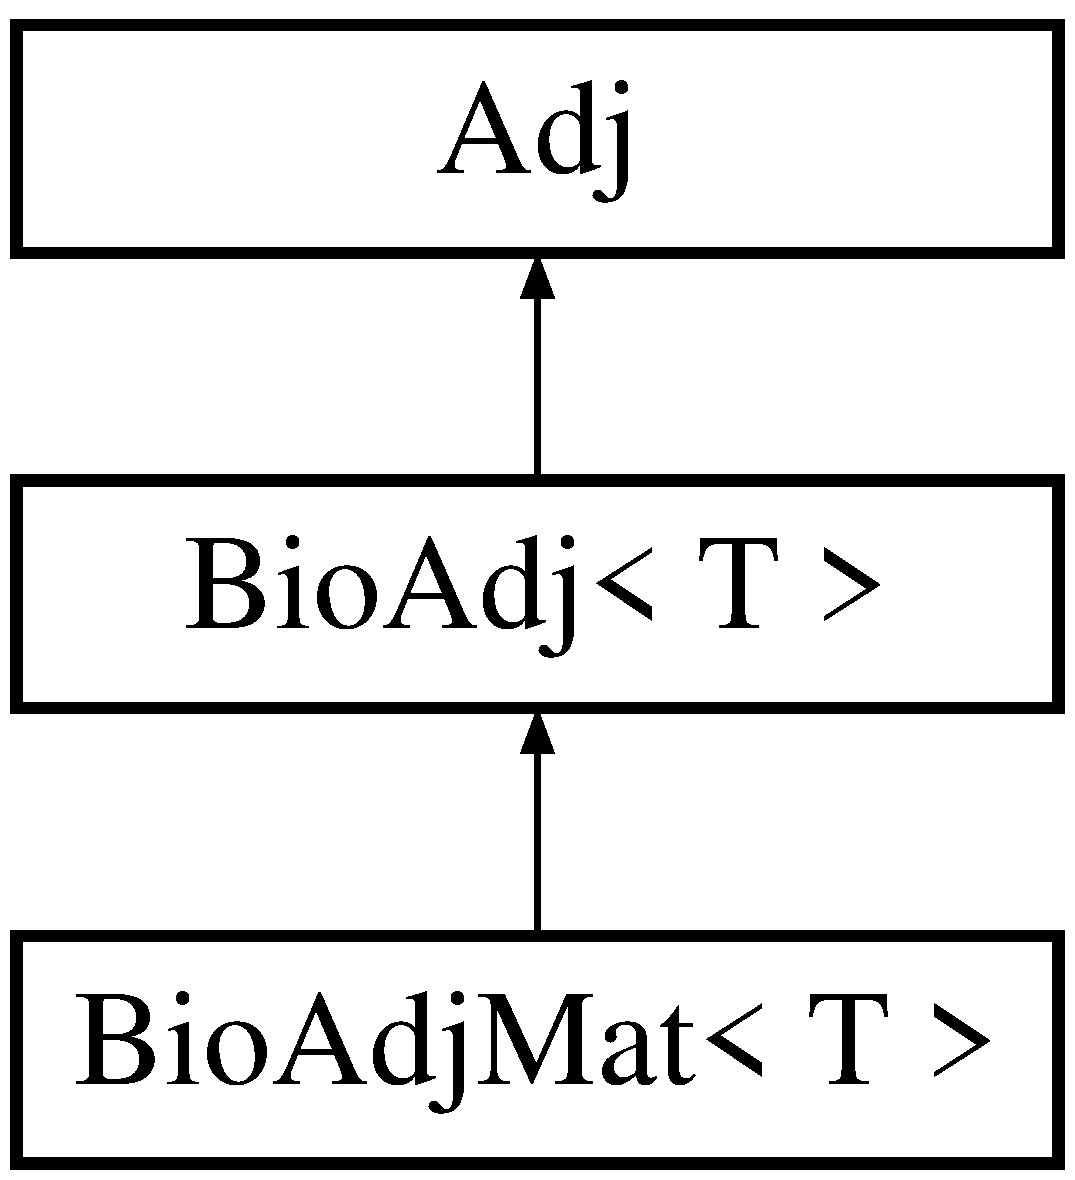
\includegraphics[height=3.000000cm]{class_bio_adj_mat}
\end{center}
\end{figure}
\subsection*{Public Member Functions}
\begin{DoxyCompactItemize}
\item 
\mbox{\Hypertarget{class_bio_adj_mat_abfaa94d4d0814a980c35ac6073397eb6}\label{class_bio_adj_mat_abfaa94d4d0814a980c35ac6073397eb6}} 
{\bfseries Bio\+Adj\+Mat} (int size=5)
\item 
\mbox{\Hypertarget{class_bio_adj_mat_a2ba626f1896a24fd77d6ba708702a7c5}\label{class_bio_adj_mat_a2ba626f1896a24fd77d6ba708702a7c5}} 
void {\bfseries set\+Edge} (const int, const int, const T)
\item 
\mbox{\Hypertarget{class_bio_adj_mat_a328e85a8522c588dbd41032824998560}\label{class_bio_adj_mat_a328e85a8522c588dbd41032824998560}} 
void {\bfseries set\+Edge} (const string \&, const string \&, const T)
\item 
\mbox{\Hypertarget{class_bio_adj_mat_a8af45dbfbe9ae88d102c4653a97eb8d7}\label{class_bio_adj_mat_a8af45dbfbe9ae88d102c4653a97eb8d7}} 
T {\bfseries get\+Edge} (const int, const int) const
\item 
\mbox{\Hypertarget{class_bio_adj_mat_af787a393b9d9ccb67fd3bd0640b7de14}\label{class_bio_adj_mat_af787a393b9d9ccb67fd3bd0640b7de14}} 
T {\bfseries get\+Edge} (const string \&, const string \&) const
\item 
\mbox{\Hypertarget{class_bio_adj_mat_ae75e3faa050519d01c17390da4e9e89c}\label{class_bio_adj_mat_ae75e3faa050519d01c17390da4e9e89c}} 
void {\bfseries set\+Node} (const int, const string \&)
\item 
\mbox{\Hypertarget{class_bio_adj_mat_a2bf70c01ef7874c1ae71566f7dfe0419}\label{class_bio_adj_mat_a2bf70c01ef7874c1ae71566f7dfe0419}} 
string {\bfseries get\+Node} (const int) const
\item 
\mbox{\Hypertarget{class_bio_adj_mat_a12b4686ed66a364465b5ce737df1372f}\label{class_bio_adj_mat_a12b4686ed66a364465b5ce737df1372f}} 
int {\bfseries size} () const
\item 
\mbox{\Hypertarget{class_bio_adj_mat_abe8ceb70c32c6d7a4e736c54beefd84c}\label{class_bio_adj_mat_abe8ceb70c32c6d7a4e736c54beefd84c}} 
void {\bfseries resize} (const int)
\item 
\mbox{\Hypertarget{class_bio_adj_mat_aae1123025ee24d47be666d35b12619b6}\label{class_bio_adj_mat_aae1123025ee24d47be666d35b12619b6}} 
T {\bfseries degree} (const int) const
\item 
\mbox{\Hypertarget{class_bio_adj_mat_a0ec8c429ca05313fb0b7050276135e13}\label{class_bio_adj_mat_a0ec8c429ca05313fb0b7050276135e13}} 
int {\bfseries number\+Of\+Edges} () const
\item 
\mbox{\Hypertarget{class_bio_adj_mat_a2313c6435a77c3f84472fd8dfab681b6}\label{class_bio_adj_mat_a2313c6435a77c3f84472fd8dfab681b6}} 
int {\bfseries find\+Node\+Index} (const string \&) const
\item 
\mbox{\Hypertarget{class_bio_adj_mat_a831ea24ad56b4ac76faa74c543c2bb41}\label{class_bio_adj_mat_a831ea24ad56b4ac76faa74c543c2bb41}} 
void {\bfseries delete\+Edge} (const string \&, const string \&)
\item 
\mbox{\Hypertarget{class_bio_adj_mat_a509ea8d9d3dc8ac4adfc9fc5fbac0caf}\label{class_bio_adj_mat_a509ea8d9d3dc8ac4adfc9fc5fbac0caf}} 
void {\bfseries delete\+Edge} (int, int)
\item 
\mbox{\Hypertarget{class_bio_adj_mat_ab47d33fad99a1b01719ba921b3e0d2c2}\label{class_bio_adj_mat_ab47d33fad99a1b01719ba921b3e0d2c2}} 
void {\bfseries delete\+Node} (const string \&)
\item 
\mbox{\Hypertarget{class_bio_adj_mat_ac3097de7d71ceee083f0766a16108e7e}\label{class_bio_adj_mat_ac3097de7d71ceee083f0766a16108e7e}} 
void {\bfseries delete\+Node} (const int)
\item 
\mbox{\Hypertarget{class_bio_adj_mat_a5c118726596cfd38c4f19418045e4a58}\label{class_bio_adj_mat_a5c118726596cfd38c4f19418045e4a58}} 
void {\bfseries copy} (const \hyperlink{class_bio_adj}{Bio\+Adj}$<$ T $>$ $\ast$rhs)
\item 
\mbox{\Hypertarget{class_bio_adj_mat_a3174456f467f1cf0d2e69acba53e6eeb}\label{class_bio_adj_mat_a3174456f467f1cf0d2e69acba53e6eeb}} 
void {\bfseries add\+Node} (const string \&a\+Node)
\item 
\mbox{\Hypertarget{class_bio_adj_mat_ab552949b392e69942dac7d5fd30d7151}\label{class_bio_adj_mat_ab552949b392e69942dac7d5fd30d7151}} 
bool {\bfseries is\+Equal} (const \hyperlink{class_bio_adj}{Bio\+Adj}$<$ T $>$ $\ast$rhs)
\item 
\mbox{\Hypertarget{class_bio_adj_mat_aaf35a2b53f4bc823a21aa2fba1c18452}\label{class_bio_adj_mat_aaf35a2b53f4bc823a21aa2fba1c18452}} 
void {\bfseries scale\+Up} (const T factor)
\item 
\mbox{\Hypertarget{class_bio_adj_mat_adb6d26f896638b79171c5af99145f5d4}\label{class_bio_adj_mat_adb6d26f896638b79171c5af99145f5d4}} 
void {\bfseries scale\+Down} (const T factor)
\end{DoxyCompactItemize}
\subsection*{Static Public Member Functions}
\begin{DoxyCompactItemize}
\item 
\mbox{\Hypertarget{class_bio_adj_mat_a12c0a3faa184d18fa08770040db50034}\label{class_bio_adj_mat_a12c0a3faa184d18fa08770040db50034}} 
static const string \& {\bfseries Network\+Type} ()
\item 
\mbox{\Hypertarget{class_bio_adj_mat_af6ec0b8518dd412025dafb082f921186}\label{class_bio_adj_mat_af6ec0b8518dd412025dafb082f921186}} 
static \hyperlink{class_adj}{Adj} $\ast$ {\bfseries make} ()
\end{DoxyCompactItemize}
\subsection*{Additional Inherited Members}


The documentation for this class was generated from the following file\+:\begin{DoxyCompactItemize}
\item 
Bio\+Adj\+Mat.\+h\end{DoxyCompactItemize}

\hypertarget{class_bio_edge}{}\section{Bio\+Edge$<$ T $>$ Class Template Reference}
\label{class_bio_edge}\index{Bio\+Edge$<$ T $>$@{Bio\+Edge$<$ T $>$}}
\subsection*{Public Member Functions}
\begin{DoxyCompactItemize}
\item 
\mbox{\Hypertarget{class_bio_edge_a4086d783935d7f70febe1d3aebe14409}\label{class_bio_edge_a4086d783935d7f70febe1d3aebe14409}} 
{\bfseries Bio\+Edge} (const T w, const string \&i, \hyperlink{class_bio_edge}{Bio\+Edge}$<$ T $>$ $\ast$n)
\item 
\mbox{\Hypertarget{class_bio_edge_ab7ec2b663698b813260003fc7cde81c2}\label{class_bio_edge_ab7ec2b663698b813260003fc7cde81c2}} 
string {\bfseries get\+Name} ()
\item 
\mbox{\Hypertarget{class_bio_edge_a6c97a0845e721c68e2a64416eef4fa2e}\label{class_bio_edge_a6c97a0845e721c68e2a64416eef4fa2e}} 
void {\bfseries set\+Name} (const string \&n)
\item 
\mbox{\Hypertarget{class_bio_edge_a114cdc0f74e9a5de8f450ba59eeebbc3}\label{class_bio_edge_a114cdc0f74e9a5de8f450ba59eeebbc3}} 
\hyperlink{class_bio_edge}{Bio\+Edge} $\ast$ {\bfseries get\+Next} ()
\item 
\mbox{\Hypertarget{class_bio_edge_ab7b6c881044bd82c5a2d370102e0786d}\label{class_bio_edge_ab7b6c881044bd82c5a2d370102e0786d}} 
void {\bfseries set\+Weight} (const float w)
\item 
\mbox{\Hypertarget{class_bio_edge_a15c1359f12ddf7c06b9585ff13313c3b}\label{class_bio_edge_a15c1359f12ddf7c06b9585ff13313c3b}} 
T {\bfseries get\+Weight} ()
\item 
\mbox{\Hypertarget{class_bio_edge_a550b29b03993989a619b2e4bf79806e3}\label{class_bio_edge_a550b29b03993989a619b2e4bf79806e3}} 
void {\bfseries set\+Next} (\hyperlink{class_bio_edge}{Bio\+Edge}$<$ T $>$ $\ast$n)
\end{DoxyCompactItemize}


The documentation for this class was generated from the following file\+:\begin{DoxyCompactItemize}
\item 
Bio\+Node.\+h\end{DoxyCompactItemize}

\hypertarget{class_bio_list}{}\section{Bio\+List$<$ T $>$ Class Template Reference}
\label{class_bio_list}\index{Bio\+List$<$ T $>$@{Bio\+List$<$ T $>$}}
\subsection*{Public Member Functions}
\begin{DoxyCompactItemize}
\item 
\mbox{\Hypertarget{class_bio_list_a99270bdf9463921b6435dcfb4e934f48}\label{class_bio_list_a99270bdf9463921b6435dcfb4e934f48}} 
{\bfseries Bio\+List} (const T weight, const string \&name)
\item 
\mbox{\Hypertarget{class_bio_list_a29cc80d0382ce4ea7d78716e50367fb7}\label{class_bio_list_a29cc80d0382ce4ea7d78716e50367fb7}} 
{\bfseries Bio\+List} (const \hyperlink{class_bio_list}{Bio\+List}$<$ T $>$ \&copy)
\item 
\mbox{\Hypertarget{class_bio_list_a02fab7396baad14645467bf22d5cc8b0}\label{class_bio_list_a02fab7396baad14645467bf22d5cc8b0}} 
{\bfseries Bio\+List} (const string \&name)
\item 
\mbox{\Hypertarget{class_bio_list_a9de2c461d7d35a9b1b16bc22e36a4454}\label{class_bio_list_a9de2c461d7d35a9b1b16bc22e36a4454}} 
bool {\bfseries search} (const string \&name)
\item 
\mbox{\Hypertarget{class_bio_list_a4eee589ab99e7ece2d2a0aed97256170}\label{class_bio_list_a4eee589ab99e7ece2d2a0aed97256170}} 
bool {\bfseries set\+Weight} (const string \&name, const T weight)
\item 
\mbox{\Hypertarget{class_bio_list_aacb7962ae1ef89c2d0f94a98c6070882}\label{class_bio_list_aacb7962ae1ef89c2d0f94a98c6070882}} 
string {\bfseries get\+Name} () const
\item 
\mbox{\Hypertarget{class_bio_list_a2598c5b263009fb1c5013b3e71a6db8a}\label{class_bio_list_a2598c5b263009fb1c5013b3e71a6db8a}} 
void {\bfseries set\+Name} (const string \&s)
\item 
\mbox{\Hypertarget{class_bio_list_af96011889bf0085140db307b294132d3}\label{class_bio_list_af96011889bf0085140db307b294132d3}} 
void {\bfseries set\+Edge\+Name} (const string \&old\+Name, const string \&new\+Name)
\item 
\mbox{\Hypertarget{class_bio_list_ad62e949ed13930d687e2cb374643a3af}\label{class_bio_list_ad62e949ed13930d687e2cb374643a3af}} 
T {\bfseries get\+Weight} (const string \&name) const
\item 
\mbox{\Hypertarget{class_bio_list_ac9accab38adbb61f19fc8b362fe3ba6e}\label{class_bio_list_ac9accab38adbb61f19fc8b362fe3ba6e}} 
\hyperlink{class_bio_edge}{Bio\+Edge}$<$ T $>$ $\ast$ {\bfseries insert\+Front} (const T weight, const string \&name)
\item 
\mbox{\Hypertarget{class_bio_list_aa5ade1fd7d850d3c66b0af9624bc48f7}\label{class_bio_list_aa5ade1fd7d850d3c66b0af9624bc48f7}} 
void {\bfseries delete\+Edge} (const string \&name)
\item 
\mbox{\Hypertarget{class_bio_list_a80f4d2798831289a23b0e7f59b146803}\label{class_bio_list_a80f4d2798831289a23b0e7f59b146803}} 
void {\bfseries clear} ()
\item 
\mbox{\Hypertarget{class_bio_list_a771e384f336e4a60a166f11e7e104455}\label{class_bio_list_a771e384f336e4a60a166f11e7e104455}} 
\hyperlink{class_bio_edge}{Bio\+Edge}$<$ T $>$ $\ast$ {\bfseries front} () const
\item 
\mbox{\Hypertarget{class_bio_list_a90e98530b5614fa49f19cef2fbcfd75f}\label{class_bio_list_a90e98530b5614fa49f19cef2fbcfd75f}} 
\hyperlink{class_bio_list}{Bio\+List}$<$ T $>$ {\bfseries operator$\ast$} (const T weight)
\item 
\mbox{\Hypertarget{class_bio_list_a5c146c21b1474fa4e6a99a27ce5722a8}\label{class_bio_list_a5c146c21b1474fa4e6a99a27ce5722a8}} 
const \hyperlink{class_bio_list}{Bio\+List}$<$ T $>$ \& {\bfseries operator$\ast$=} (const T weight)
\item 
\mbox{\Hypertarget{class_bio_list_a55385168b85f8a34715d2c03a1fe4a3b}\label{class_bio_list_a55385168b85f8a34715d2c03a1fe4a3b}} 
\hyperlink{class_bio_list}{Bio\+List}$<$ T $>$ {\bfseries operator/} (const T weight)
\item 
\mbox{\Hypertarget{class_bio_list_a551599a405b18e3e2987f8c04a8a68c8}\label{class_bio_list_a551599a405b18e3e2987f8c04a8a68c8}} 
const \hyperlink{class_bio_list}{Bio\+List}$<$ T $>$ \& {\bfseries operator/=} (const T weight)
\end{DoxyCompactItemize}


The documentation for this class was generated from the following file\+:\begin{DoxyCompactItemize}
\item 
Bio\+List.\+h\end{DoxyCompactItemize}

\hypertarget{class_bio_net}{}\section{Bio\+Net$<$ T $>$ Class Template Reference}
\label{class_bio_net}\index{Bio\+Net$<$ T $>$@{Bio\+Net$<$ T $>$}}
\subsection*{Public Member Functions}
\begin{DoxyCompactItemize}
\item 
\mbox{\Hypertarget{class_bio_net_af18d85c34aa8d04e8ddea94c256b2ac6}\label{class_bio_net_af18d85c34aa8d04e8ddea94c256b2ac6}} 
{\bfseries Bio\+Net} (const T, const T, const bool=false, const string \&=\hyperlink{class_bio_adj_mat}{Bio\+Adj\+Mat}$<$ float $>$\+::Network\+Type())
\item 
\mbox{\Hypertarget{class_bio_net_a6ac93ccd7e25a7de6acbfd3af0355a67}\label{class_bio_net_a6ac93ccd7e25a7de6acbfd3af0355a67}} 
{\bfseries Bio\+Net} (const \hyperlink{class_bio_net}{Bio\+Net}$<$ T $>$ \&)
\item 
\mbox{\Hypertarget{class_bio_net_a0775e0b7bfa4f50c6ff595f915d00c69}\label{class_bio_net_a0775e0b7bfa4f50c6ff595f915d00c69}} 
{\bfseries Bio\+Net} (\hyperlink{class_bio_net}{Bio\+Net}$<$ T $>$ \&\&)
\item 
\mbox{\Hypertarget{class_bio_net_a51934a34817c3dab71e6a796e02f9850}\label{class_bio_net_a51934a34817c3dab71e6a796e02f9850}} 
void {\bfseries set\+Range} (const T, const T)
\item 
\mbox{\Hypertarget{class_bio_net_a255b8c04b7ebb8acf164ecd66cfd2e2c}\label{class_bio_net_a255b8c04b7ebb8acf164ecd66cfd2e2c}} 
void {\bfseries set\+Edge} (const int, const int, const T)
\item 
\mbox{\Hypertarget{class_bio_net_a91d6454117016366898cb40c43cb6fd5}\label{class_bio_net_a91d6454117016366898cb40c43cb6fd5}} 
void {\bfseries set\+Node} (const int, const string \&n)
\item 
\mbox{\Hypertarget{class_bio_net_af3b15d9a7e155670b906dd6cb4c03fc4}\label{class_bio_net_af3b15d9a7e155670b906dd6cb4c03fc4}} 
void {\bfseries delete\+Edge} (const int, const int)
\item 
\mbox{\Hypertarget{class_bio_net_a78d341c6d9fade83aec1bcb569d02909}\label{class_bio_net_a78d341c6d9fade83aec1bcb569d02909}} 
void {\bfseries delete\+Edge} (const string \&l, const string \&r)
\item 
\mbox{\Hypertarget{class_bio_net_a9dc1a7c48aa9078413c96d2f39ef0c0d}\label{class_bio_net_a9dc1a7c48aa9078413c96d2f39ef0c0d}} 
const T {\bfseries shortest\+Path} (const int, const int) const
\item 
\mbox{\Hypertarget{class_bio_net_a77de66d6eb37a030fc4f50670e9cd5f1}\label{class_bio_net_a77de66d6eb37a030fc4f50670e9cd5f1}} 
void {\bfseries resize} (const int size)
\item 
\mbox{\Hypertarget{class_bio_net_a7b85dcaa5264318e144dde4cfe3819af}\label{class_bio_net_a7b85dcaa5264318e144dde4cfe3819af}} 
void {\bfseries clear} ()
\item 
\mbox{\Hypertarget{class_bio_net_a3c6903721152c55f134d15d64868e1d1}\label{class_bio_net_a3c6903721152c55f134d15d64868e1d1}} 
const T {\bfseries get\+Edge} (const int, const int) const
\item 
\mbox{\Hypertarget{class_bio_net_ab174f91c9fb28e5ce0a1c99ab94f3296}\label{class_bio_net_ab174f91c9fb28e5ce0a1c99ab94f3296}} 
const string {\bfseries get\+Node} (const int) const
\item 
\mbox{\Hypertarget{class_bio_net_ad62beca214bbd54dd3f250beb99532f9}\label{class_bio_net_ad62beca214bbd54dd3f250beb99532f9}} 
const T {\bfseries get\+Min\+Weight} () const
\item 
\mbox{\Hypertarget{class_bio_net_a21d1879301feaa1c1a8f2b1d8ed82d6d}\label{class_bio_net_a21d1879301feaa1c1a8f2b1d8ed82d6d}} 
const T {\bfseries get\+Max\+Weight} () const
\item 
\mbox{\Hypertarget{class_bio_net_ac0563308f147e9006f738ec3798e9fa9}\label{class_bio_net_ac0563308f147e9006f738ec3798e9fa9}} 
const std\+::string \& {\bfseries get\+Network\+Type} () const
\item 
\mbox{\Hypertarget{class_bio_net_a281c9319ff7017570be6e2e880af8b43}\label{class_bio_net_a281c9319ff7017570be6e2e880af8b43}} 
const string \& {\bfseries operator\mbox{[}$\,$\mbox{]}} (size\+\_\+t index) const
\item 
\mbox{\Hypertarget{class_bio_net_a14e7e57741f35c5878f2d233e19dab98}\label{class_bio_net_a14e7e57741f35c5878f2d233e19dab98}} 
const T {\bfseries operator()} (size\+\_\+t lhs, size\+\_\+t rhs) const
\item 
\mbox{\Hypertarget{class_bio_net_aad6bff84a85602a8a981e67ce47d73f7}\label{class_bio_net_aad6bff84a85602a8a981e67ce47d73f7}} 
const T {\bfseries operator()} (const string \&lhs, const string \&rhs) const
\item 
\mbox{\Hypertarget{class_bio_net_a710924bcbc04475b16aea6cdd1f11697}\label{class_bio_net_a710924bcbc04475b16aea6cdd1f11697}} 
\hyperlink{class_bio_net}{Bio\+Net}$<$ T $>$ {\bfseries operator+} (const string \&rhs) const
\item 
\mbox{\Hypertarget{class_bio_net_a01a34fc724da95f508b1edb1b010545b}\label{class_bio_net_a01a34fc724da95f508b1edb1b010545b}} 
const \hyperlink{class_bio_net}{Bio\+Net}$<$ T $>$ \& {\bfseries operator+=} (const string \&)
\item 
\mbox{\Hypertarget{class_bio_net_a59581ba7ddaf2b80a6d2478d71c958d5}\label{class_bio_net_a59581ba7ddaf2b80a6d2478d71c958d5}} 
const \hyperlink{class_bio_net}{Bio\+Net}$<$ T $>$ \& {\bfseries operator=} (const \hyperlink{class_bio_net}{Bio\+Net} \&rhs)
\item 
\mbox{\Hypertarget{class_bio_net_a689664558c94713b40f78fa67670f355}\label{class_bio_net_a689664558c94713b40f78fa67670f355}} 
const bool {\bfseries operator==} (const \hyperlink{class_bio_net}{Bio\+Net} \&rhs) const
\item 
\mbox{\Hypertarget{class_bio_net_a62efbcf64a6e7cb1070e3fb7aeb1ff83}\label{class_bio_net_a62efbcf64a6e7cb1070e3fb7aeb1ff83}} 
const bool {\bfseries operator!=} (const \hyperlink{class_bio_net}{Bio\+Net} \&rhs) const
\item 
\mbox{\Hypertarget{class_bio_net_a4062376b7be85486baaaa110c1912423}\label{class_bio_net_a4062376b7be85486baaaa110c1912423}} 
{\footnotesize template$<$class R $>$ }\\const \hyperlink{class_bio_net}{Bio\+Net}$<$ T $>$ \& {\bfseries operator=} (const \hyperlink{class_bio_net}{Bio\+Net}$<$ R $>$ \&rhs)
\item 
\mbox{\Hypertarget{class_bio_net_adfebac99ed2809f3d3cf62a5727f0e9a}\label{class_bio_net_adfebac99ed2809f3d3cf62a5727f0e9a}} 
ostream \& {\bfseries operator$<$$<$} (ostream \&) const
\item 
\mbox{\Hypertarget{class_bio_net_ab6d1e15ea52cb798da5d1eefec035e4d}\label{class_bio_net_ab6d1e15ea52cb798da5d1eefec035e4d}} 
{\footnotesize template$<$class T $>$ }\\const \hyperlink{class_bio_net}{Bio\+Net}$<$ T $>$ \& {\bfseries operator+=} (const string \&rhs)
\item 
\mbox{\Hypertarget{class_bio_net_af14fa0464ce7943468ff42b48a13807e}\label{class_bio_net_af14fa0464ce7943468ff42b48a13807e}} 
{\footnotesize template$<$class T $>$ }\\\hyperlink{class_bio_net}{Bio\+Net}$<$ T $>$ {\bfseries operator+} (const string \&rhs) const
\item 
\mbox{\Hypertarget{class_bio_net_aa4e9fb16fa8b98eaf2ba5731d4437aa7}\label{class_bio_net_aa4e9fb16fa8b98eaf2ba5731d4437aa7}} 
\hyperlink{class_bio_net}{Bio\+Net}$<$ T $>$ {\bfseries operator$\ast$} (const T) const
\item 
\mbox{\Hypertarget{class_bio_net_af29d2f7582b887fa98884a0107f7e6b0}\label{class_bio_net_af29d2f7582b887fa98884a0107f7e6b0}} 
const \hyperlink{class_bio_net}{Bio\+Net}$<$ T $>$ \& {\bfseries operator$\ast$=} (const T) const
\item 
\mbox{\Hypertarget{class_bio_net_a985192f23c7b5e209d191a47b9aab9e2}\label{class_bio_net_a985192f23c7b5e209d191a47b9aab9e2}} 
\hyperlink{class_bio_net}{Bio\+Net}$<$ T $>$ {\bfseries operator/} (const T) const
\item 
\mbox{\Hypertarget{class_bio_net_a2367e25a99097d4704d86ad34a4af8df}\label{class_bio_net_a2367e25a99097d4704d86ad34a4af8df}} 
const \hyperlink{class_bio_net}{Bio\+Net}$<$ T $>$ \& {\bfseries operator/=} (const T) const
\item 
\mbox{\Hypertarget{class_bio_net_a7eb4a3c1731c8883a8f34762f51d4951}\label{class_bio_net_a7eb4a3c1731c8883a8f34762f51d4951}} 
void {\bfseries convert\+To\+Type} (const string \&)
\item 
\mbox{\Hypertarget{class_bio_net_a551ed339a1ee3cf82d39e29db72fbcbe}\label{class_bio_net_a551ed339a1ee3cf82d39e29db72fbcbe}} 
const T {\bfseries degree} (const int) const
\item 
\mbox{\Hypertarget{class_bio_net_ab8b612b8dd76b0e7930ea65aff1726b4}\label{class_bio_net_ab8b612b8dd76b0e7930ea65aff1726b4}} 
const size\+\_\+t {\bfseries size} () const
\item 
\mbox{\Hypertarget{class_bio_net_a91bb601d635f33d199f267f37853e9e5}\label{class_bio_net_a91bb601d635f33d199f267f37853e9e5}} 
const int {\bfseries number\+Of\+Edges} () const
\end{DoxyCompactItemize}


The documentation for this class was generated from the following file\+:\begin{DoxyCompactItemize}
\item 
Bio\+Net.\+h\end{DoxyCompactItemize}

\hypertarget{class_bio_net_exception}{}\section{Bio\+Net\+Exception Class Reference}
\label{class_bio_net_exception}\index{Bio\+Net\+Exception@{Bio\+Net\+Exception}}
Inheritance diagram for Bio\+Net\+Exception\+:\begin{figure}[H]
\begin{center}
\leavevmode
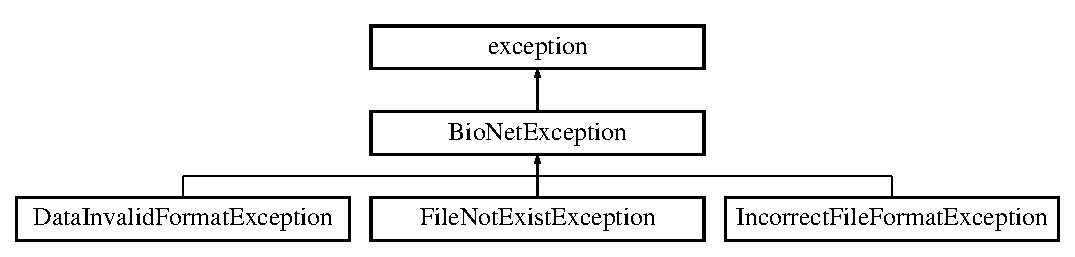
\includegraphics[height=3.000000cm]{class_bio_net_exception}
\end{center}
\end{figure}
\subsection*{Public Member Functions}
\begin{DoxyCompactItemize}
\item 
\mbox{\Hypertarget{class_bio_net_exception_a2b4059297de2d45bc15ce0f4de16c068}\label{class_bio_net_exception_a2b4059297de2d45bc15ce0f4de16c068}} 
{\bfseries Bio\+Net\+Exception} (const std\+::string \&m)
\item 
\mbox{\Hypertarget{class_bio_net_exception_a14478e246d477f427a849276ab61f775}\label{class_bio_net_exception_a14478e246d477f427a849276ab61f775}} 
const char $\ast$ {\bfseries what} () const  throw ()
\end{DoxyCompactItemize}


The documentation for this class was generated from the following files\+:\begin{DoxyCompactItemize}
\item 
Bio\+Net\+Exception.\+h\item 
Bio\+Net\+Exception.\+cpp\end{DoxyCompactItemize}

\hypertarget{class_c_s_v_reader}{}\section{C\+S\+V\+Reader Class Reference}
\label{class_c_s_v_reader}\index{C\+S\+V\+Reader@{C\+S\+V\+Reader}}
\subsection*{Static Public Member Functions}
\begin{DoxyCompactItemize}
\item 
\mbox{\Hypertarget{class_c_s_v_reader_acbec14efb05c8de0e406a55c56b85fe8}\label{class_c_s_v_reader_acbec14efb05c8de0e406a55c56b85fe8}} 
{\footnotesize template$<$typename T $>$ }\\static void {\bfseries do\+Read} (\hyperlink{class_bio_net}{Bio\+Net}$<$ T $>$ \&bionet, const string \&fname)
\item 
\mbox{\Hypertarget{class_c_s_v_reader_ae7e9cddd52db8db7cc806c9d05e74fa7}\label{class_c_s_v_reader_ae7e9cddd52db8db7cc806c9d05e74fa7}} 
{\footnotesize template$<$typename T $>$ }\\static void {\bfseries do\+Write} (\hyperlink{class_bio_net}{Bio\+Net}$<$ T $>$ \&file, const string \&fname)
\item 
\mbox{\Hypertarget{class_c_s_v_reader_a09e765b08b39a037268a7a31b8729cf7}\label{class_c_s_v_reader_a09e765b08b39a037268a7a31b8729cf7}} 
static string {\bfseries get\+Default\+Ext} ()
\end{DoxyCompactItemize}


The documentation for this class was generated from the following files\+:\begin{DoxyCompactItemize}
\item 
Turing/\+Turing/C\+S\+V\+Reader.\+h\item 
Turing/\+Turing/C\+S\+V\+Reader.\+cpp\end{DoxyCompactItemize}

\hypertarget{class_data_invalid_format_exception}{}\section{Data\+Invalid\+Format\+Exception Class Reference}
\label{class_data_invalid_format_exception}\index{Data\+Invalid\+Format\+Exception@{Data\+Invalid\+Format\+Exception}}
Inheritance diagram for Data\+Invalid\+Format\+Exception\+:\begin{figure}[H]
\begin{center}
\leavevmode
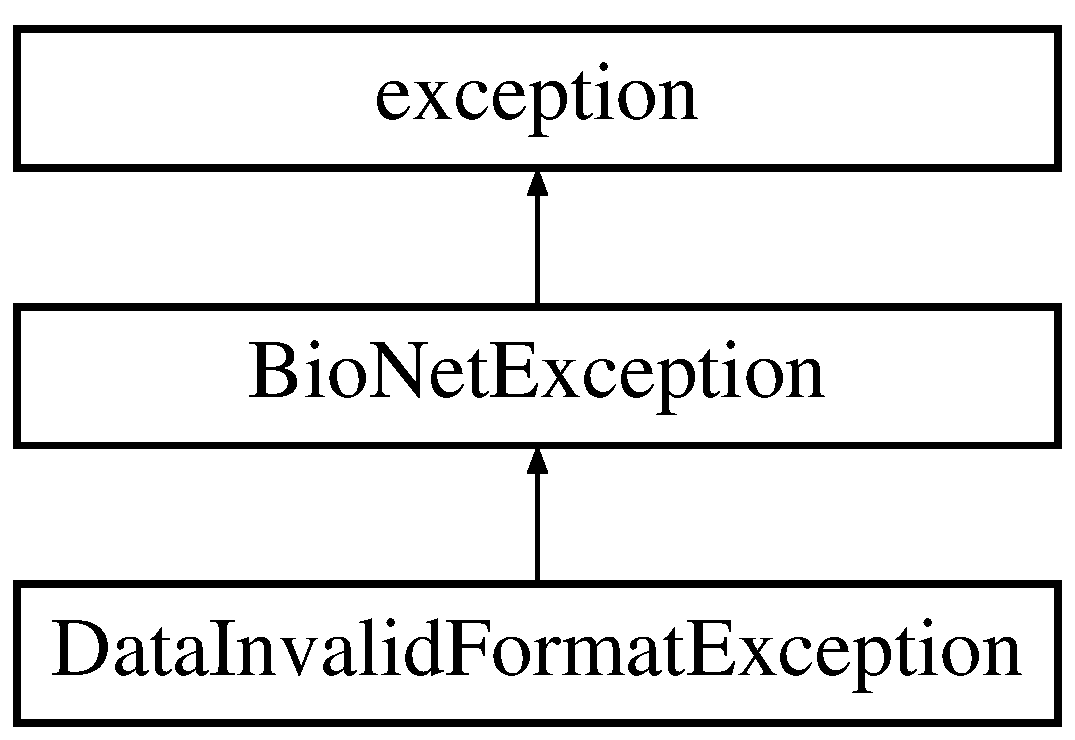
\includegraphics[height=3.000000cm]{class_data_invalid_format_exception}
\end{center}
\end{figure}
\subsection*{Public Member Functions}
\begin{DoxyCompactItemize}
\item 
\mbox{\Hypertarget{class_data_invalid_format_exception_a2d5a420fffae751946eb0750486a238f}\label{class_data_invalid_format_exception_a2d5a420fffae751946eb0750486a238f}} 
{\bfseries Data\+Invalid\+Format\+Exception} (string message)
\end{DoxyCompactItemize}


The documentation for this class was generated from the following file\+:\begin{DoxyCompactItemize}
\item 
Knuth/\+Knuth/Exception.\+h\end{DoxyCompactItemize}

\hypertarget{struct_edge}{}\section{Edge Struct Reference}
\label{struct_edge}\index{Edge@{Edge}}
\subsection*{Public Attributes}
\begin{DoxyCompactItemize}
\item 
\mbox{\Hypertarget{struct_edge_adcf410ae923d69e22ede2cd59ee80108}\label{struct_edge_adcf410ae923d69e22ede2cd59ee80108}} 
int {\bfseries source}
\item 
\mbox{\Hypertarget{struct_edge_aa39574b7bb4de6b41acd5c5c3d6331cc}\label{struct_edge_aa39574b7bb4de6b41acd5c5c3d6331cc}} 
int {\bfseries target}
\item 
\mbox{\Hypertarget{struct_edge_a6d0148402e635354c03a151c77fcbdd8}\label{struct_edge_a6d0148402e635354c03a151c77fcbdd8}} 
double {\bfseries weight}
\end{DoxyCompactItemize}


The documentation for this struct was generated from the following file\+:\begin{DoxyCompactItemize}
\item 
Knuth/\+Knuth/G\+M\+L\+Reader.\+h\end{DoxyCompactItemize}

\hypertarget{class_file_handler}{}\section{File\+Handler Class Reference}
\label{class_file_handler}\index{File\+Handler@{File\+Handler}}
Inheritance diagram for File\+Handler\+:\begin{figure}[H]
\begin{center}
\leavevmode
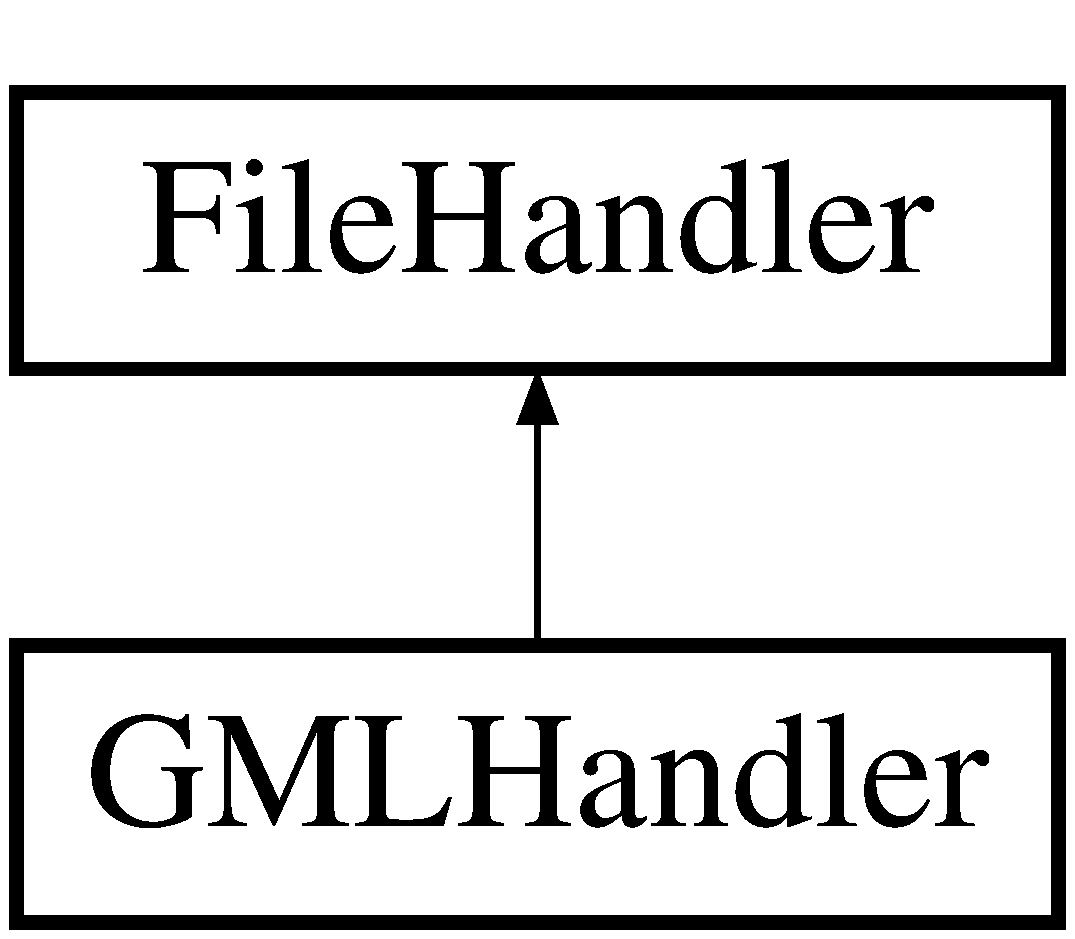
\includegraphics[height=2.000000cm]{class_file_handler}
\end{center}
\end{figure}
\subsection*{Public Member Functions}
\begin{DoxyCompactItemize}
\item 
\mbox{\Hypertarget{class_file_handler_ae098390e45e1cf994e9ec9c713090fbd}\label{class_file_handler_ae098390e45e1cf994e9ec9c713090fbd}} 
string {\bfseries get\+Default\+Ext} ()
\end{DoxyCompactItemize}
\subsection*{Protected Attributes}
\begin{DoxyCompactItemize}
\item 
\mbox{\Hypertarget{class_file_handler_a39b055806a5514f19ba6efe1a3f9ccfa}\label{class_file_handler_a39b055806a5514f19ba6efe1a3f9ccfa}} 
string {\bfseries extension}
\end{DoxyCompactItemize}


The documentation for this class was generated from the following file\+:\begin{DoxyCompactItemize}
\item 
File.\+h\end{DoxyCompactItemize}

\hypertarget{class_file_not_exist_exception}{}\section{File\+Not\+Exist\+Exception Class Reference}
\label{class_file_not_exist_exception}\index{File\+Not\+Exist\+Exception@{File\+Not\+Exist\+Exception}}
Inheritance diagram for File\+Not\+Exist\+Exception\+:\begin{figure}[H]
\begin{center}
\leavevmode
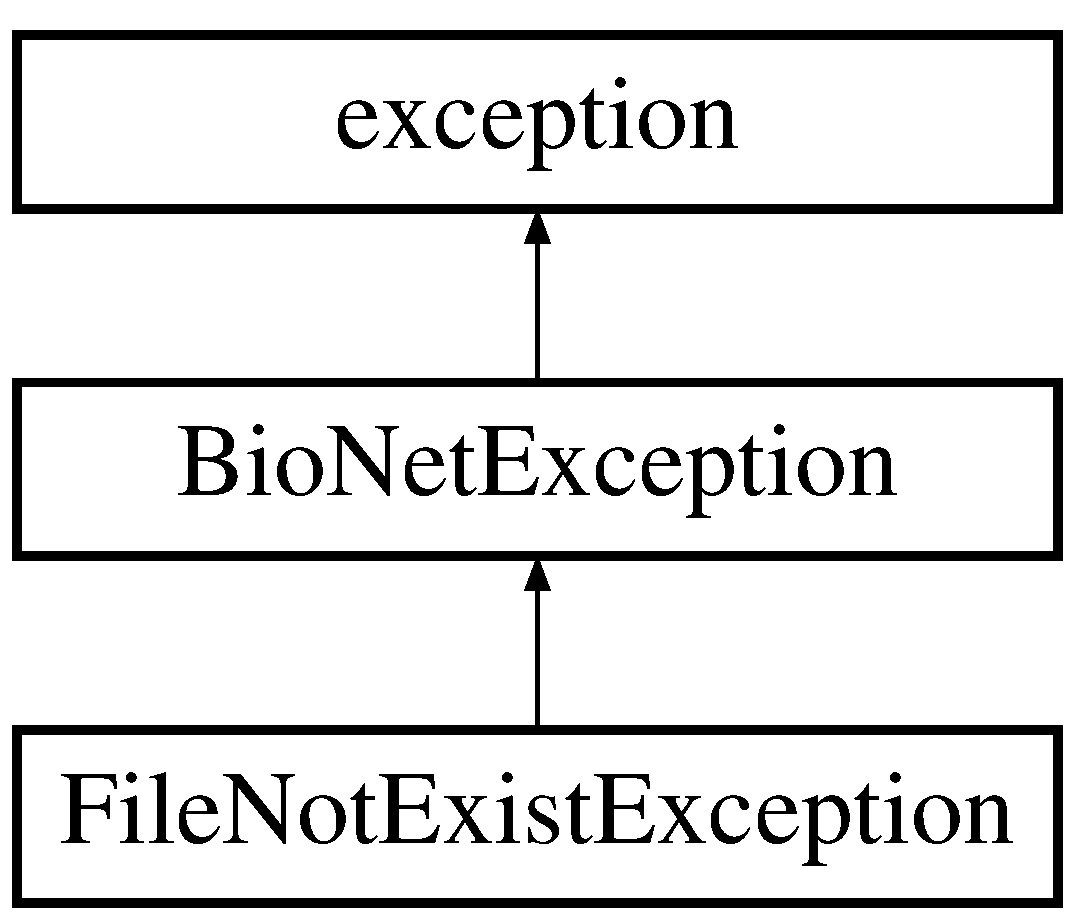
\includegraphics[height=3.000000cm]{class_file_not_exist_exception}
\end{center}
\end{figure}
\subsection*{Public Member Functions}
\begin{DoxyCompactItemize}
\item 
\mbox{\Hypertarget{class_file_not_exist_exception_ac7c9910c68ba73381f8e04ed1cc1c455}\label{class_file_not_exist_exception_ac7c9910c68ba73381f8e04ed1cc1c455}} 
{\bfseries File\+Not\+Exist\+Exception} (string message)
\end{DoxyCompactItemize}


The documentation for this class was generated from the following file\+:\begin{DoxyCompactItemize}
\item 
Knuth/\+Knuth/Exception.\+h\end{DoxyCompactItemize}

\hypertarget{class_g_m_l_handler}{}\section{G\+M\+L\+Handler Class Reference}
\label{class_g_m_l_handler}\index{G\+M\+L\+Handler@{G\+M\+L\+Handler}}
Inheritance diagram for G\+M\+L\+Handler\+:\begin{figure}[H]
\begin{center}
\leavevmode
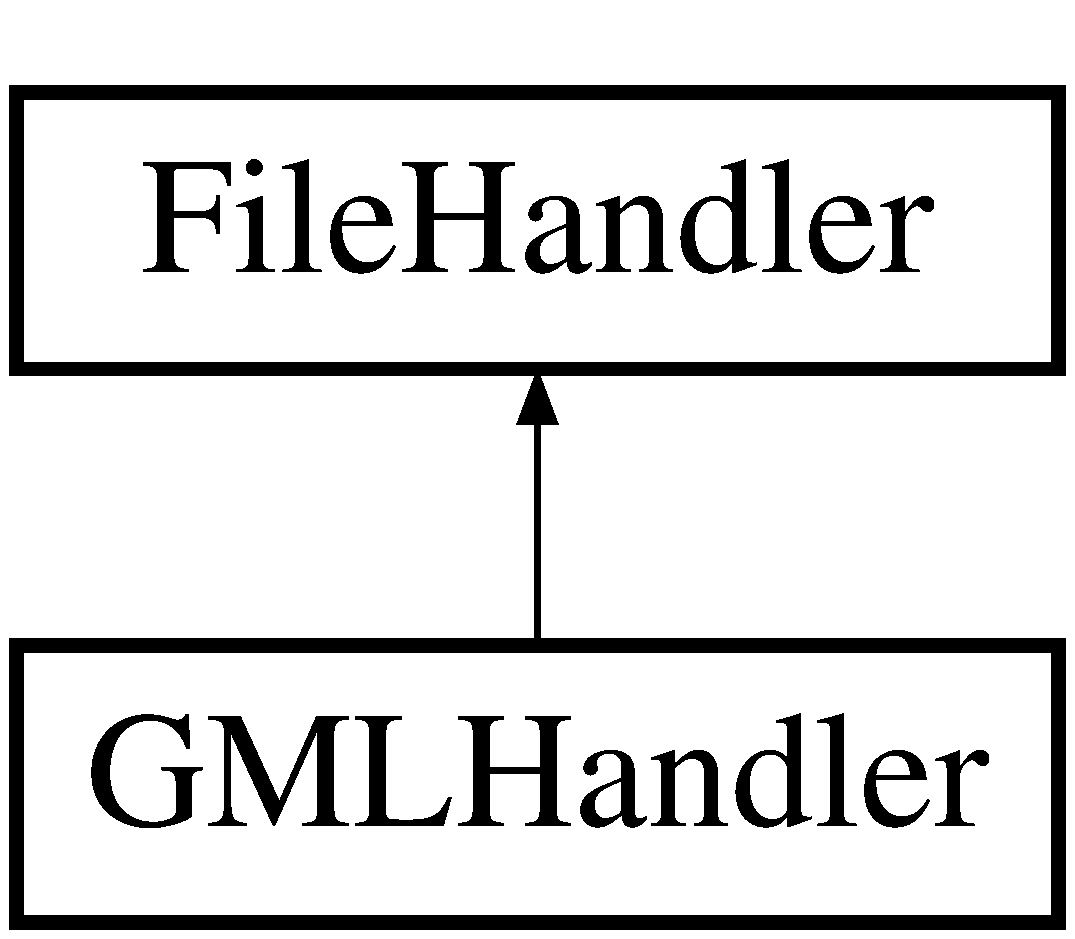
\includegraphics[height=2.000000cm]{class_g_m_l_handler}
\end{center}
\end{figure}
\subsection*{Static Public Member Functions}
\begin{DoxyCompactItemize}
\item 
\mbox{\Hypertarget{class_g_m_l_handler_a421ba270909a741ba0cfa0e9ea1a0193}\label{class_g_m_l_handler_a421ba270909a741ba0cfa0e9ea1a0193}} 
{\footnotesize template$<$typename T $>$ }\\static void {\bfseries do\+Read} (\hyperlink{class_bio_net}{Bio\+Net}$<$ T $>$ \&, const string \&fname)
\item 
\mbox{\Hypertarget{class_g_m_l_handler_a94591c1af1a83cc546216553bc95d01a}\label{class_g_m_l_handler_a94591c1af1a83cc546216553bc95d01a}} 
{\footnotesize template$<$typename T $>$ }\\static void {\bfseries do\+Write} (\hyperlink{class_bio_net}{Bio\+Net}$<$ T $>$ \&, const string \&fname)
\end{DoxyCompactItemize}
\subsection*{Additional Inherited Members}


The documentation for this class was generated from the following files\+:\begin{DoxyCompactItemize}
\item 
Knuth/\+Knuth/G\+M\+L\+Reader.\+h\item 
Knuth/\+Knuth/G\+M\+L\+Reader.\+cpp\end{DoxyCompactItemize}

\hypertarget{class_incorrect_file_format_exception}{}\section{Incorrect\+File\+Format\+Exception Class Reference}
\label{class_incorrect_file_format_exception}\index{Incorrect\+File\+Format\+Exception@{Incorrect\+File\+Format\+Exception}}
Inheritance diagram for Incorrect\+File\+Format\+Exception\+:\begin{figure}[H]
\begin{center}
\leavevmode
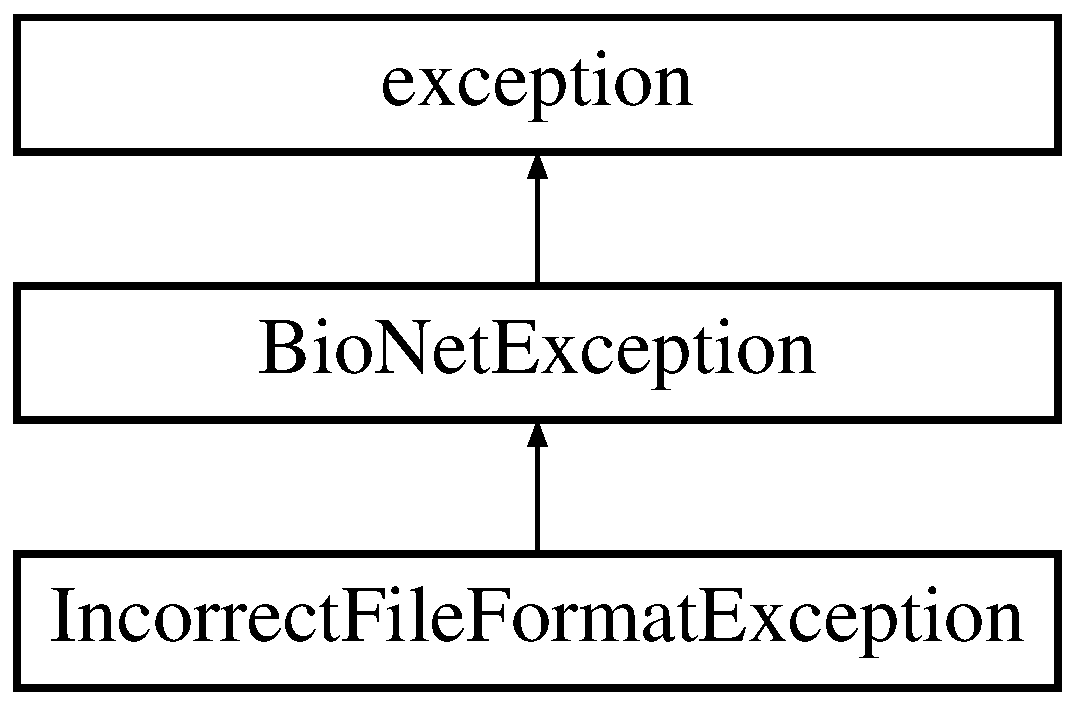
\includegraphics[height=3.000000cm]{class_incorrect_file_format_exception}
\end{center}
\end{figure}
\subsection*{Public Member Functions}
\begin{DoxyCompactItemize}
\item 
\mbox{\Hypertarget{class_incorrect_file_format_exception_aa7a1beea854053882117309870d7e9ca}\label{class_incorrect_file_format_exception_aa7a1beea854053882117309870d7e9ca}} 
{\bfseries Incorrect\+File\+Format\+Exception} (string message)
\end{DoxyCompactItemize}


The documentation for this class was generated from the following file\+:\begin{DoxyCompactItemize}
\item 
Knuth/\+Knuth/Exception.\+h\end{DoxyCompactItemize}

\hypertarget{class_i_o}{}\section{IO Class Reference}
\label{class_i_o}\index{IO@{IO}}
Inheritance diagram for IO\+:\begin{figure}[H]
\begin{center}
\leavevmode
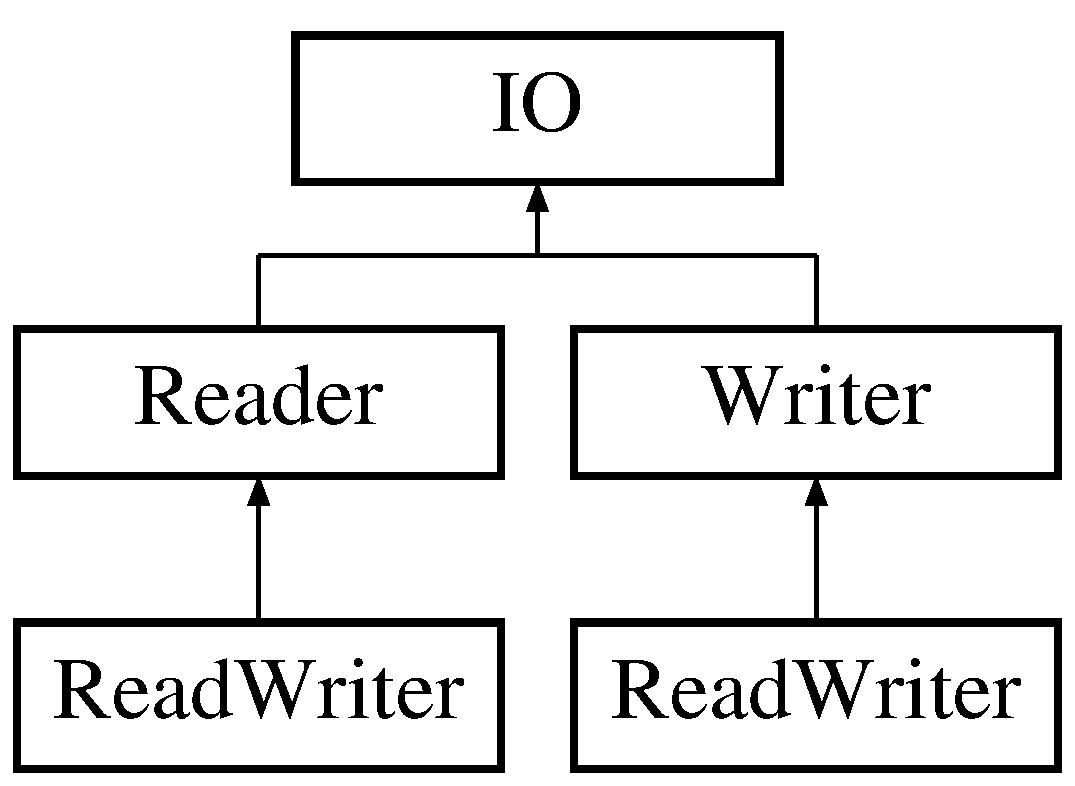
\includegraphics[height=3.000000cm]{class_i_o}
\end{center}
\end{figure}
\subsection*{Public Member Functions}
\begin{DoxyCompactItemize}
\item 
\mbox{\Hypertarget{class_i_o_ae8ab594ad6f653b7552fda638eec63a8}\label{class_i_o_ae8ab594ad6f653b7552fda638eec63a8}} 
{\bfseries IO} (string path=\char`\"{}C\+:\textbackslash{}sers\textbackslash{}tudent\textbackslash{}esktop\textbackslash{}io\+Net\textbackslash{}ata\textbackslash{}asic\textbackslash{}hree\+\_\+triads\textbackslash{})
\end{DoxyCompactItemize}
\subsection*{Static Public Member Functions}
\begin{DoxyCompactItemize}
\item 
\mbox{\Hypertarget{class_i_o_af6385db5958f04392a7986fbf4af16db}\label{class_i_o_af6385db5958f04392a7986fbf4af16db}} 
static string {\bfseries get\+Default\+Path} ()
\item 
\mbox{\Hypertarget{class_i_o_a66ac356bf3ace0c37f1fccf6d3d1359c}\label{class_i_o_a66ac356bf3ace0c37f1fccf6d3d1359c}} 
static void {\bfseries set\+Default\+Path} (string p)
\end{DoxyCompactItemize}
\subsection*{Static Protected Attributes}
\begin{DoxyCompactItemize}
\item 
\mbox{\Hypertarget{class_i_o_afe39579558a542005c1be707e23abad0}\label{class_i_o_afe39579558a542005c1be707e23abad0}} 
static string {\bfseries default\+Path} = \char`\"{}C\+:\textbackslash{}\textbackslash{}\+Users\textbackslash{}\textbackslash{}student\textbackslash{}\textbackslash{}\+Desktop\textbackslash{}\textbackslash{}\+Bio\+Net\textbackslash{}\textbackslash{}data\textbackslash{}\textbackslash{}\+Basic\textbackslash{}\textbackslash{}three\+\_\+triads\textbackslash{}\textbackslash{}\char`\"{}
\end{DoxyCompactItemize}


The documentation for this class was generated from the following files\+:\begin{DoxyCompactItemize}
\item 
I\+O.\+h\item 
I\+O.\+cpp\end{DoxyCompactItemize}

\hypertarget{struct_node}{}\section{Node Struct Reference}
\label{struct_node}\index{Node@{Node}}
\subsection*{Public Attributes}
\begin{DoxyCompactItemize}
\item 
\mbox{\Hypertarget{struct_node_a59a543130a10c95f1e8642cf8c5645e8}\label{struct_node_a59a543130a10c95f1e8642cf8c5645e8}} 
int {\bfseries id}
\item 
\mbox{\Hypertarget{struct_node_a303618c90c74231cce2c097e3fdb7f02}\label{struct_node_a303618c90c74231cce2c097e3fdb7f02}} 
string {\bfseries label}
\end{DoxyCompactItemize}


The documentation for this struct was generated from the following file\+:\begin{DoxyCompactItemize}
\item 
Knuth/\+Knuth/G\+M\+L\+Reader.\+h\end{DoxyCompactItemize}

\hypertarget{class_reader}{}\section{Reader Class Reference}
\label{class_reader}\index{Reader@{Reader}}
Inheritance diagram for Reader\+:\begin{figure}[H]
\begin{center}
\leavevmode
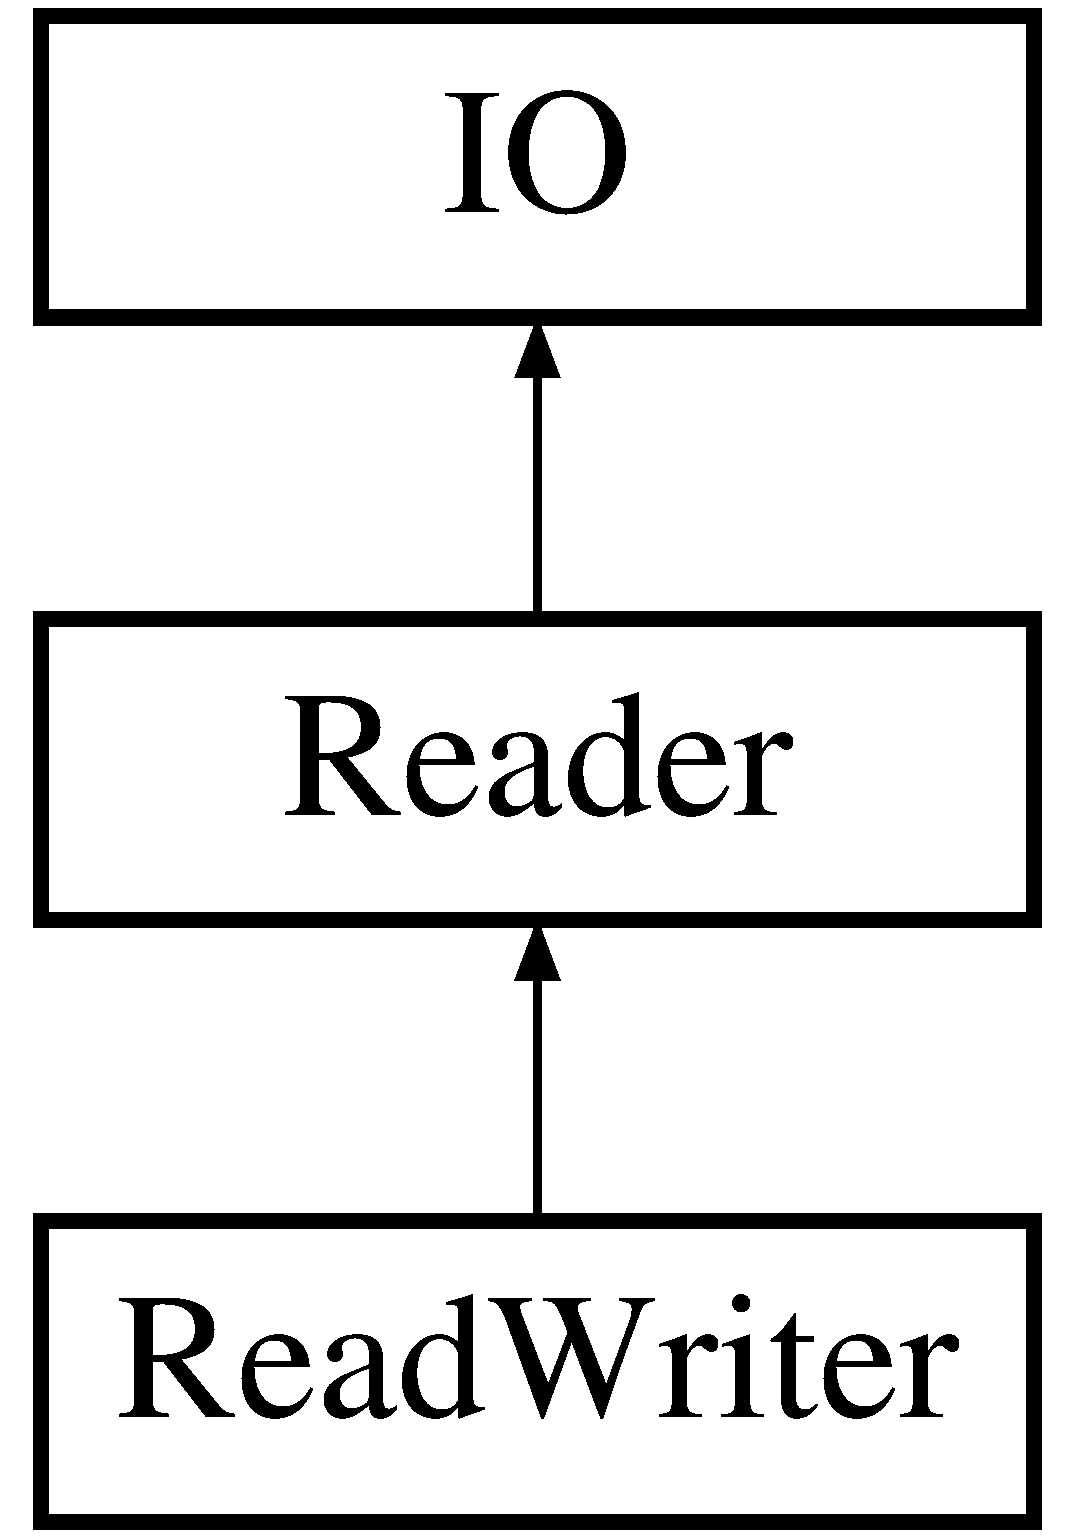
\includegraphics[height=3.000000cm]{class_reader}
\end{center}
\end{figure}
\subsection*{Public Member Functions}
\begin{DoxyCompactItemize}
\item 
\mbox{\Hypertarget{class_reader_ae6cad7214cf6b6a26fb48a650f8dd8b3}\label{class_reader_ae6cad7214cf6b6a26fb48a650f8dd8b3}} 
{\bfseries Reader} (string p=I\+O\+::get\+Default\+Path())
\end{DoxyCompactItemize}
\subsection*{Static Public Member Functions}
\begin{DoxyCompactItemize}
\item 
\mbox{\Hypertarget{class_reader_a455679a18e5019c366a3b409171a358e}\label{class_reader_a455679a18e5019c366a3b409171a358e}} 
{\footnotesize template$<$class R , class T $>$ }\\static void {\bfseries read\+File} (\hyperlink{class_bio_net}{Bio\+Net}$<$ T $>$ \&bn, string \&fname, bool use\+Default=true)
\end{DoxyCompactItemize}
\subsection*{Additional Inherited Members}


The documentation for this class was generated from the following file\+:\begin{DoxyCompactItemize}
\item 
Reader.\+h\end{DoxyCompactItemize}

\hypertarget{class_read_writer}{}\section{Read\+Writer Class Reference}
\label{class_read_writer}\index{Read\+Writer@{Read\+Writer}}
Inheritance diagram for Read\+Writer\+:\begin{figure}[H]
\begin{center}
\leavevmode
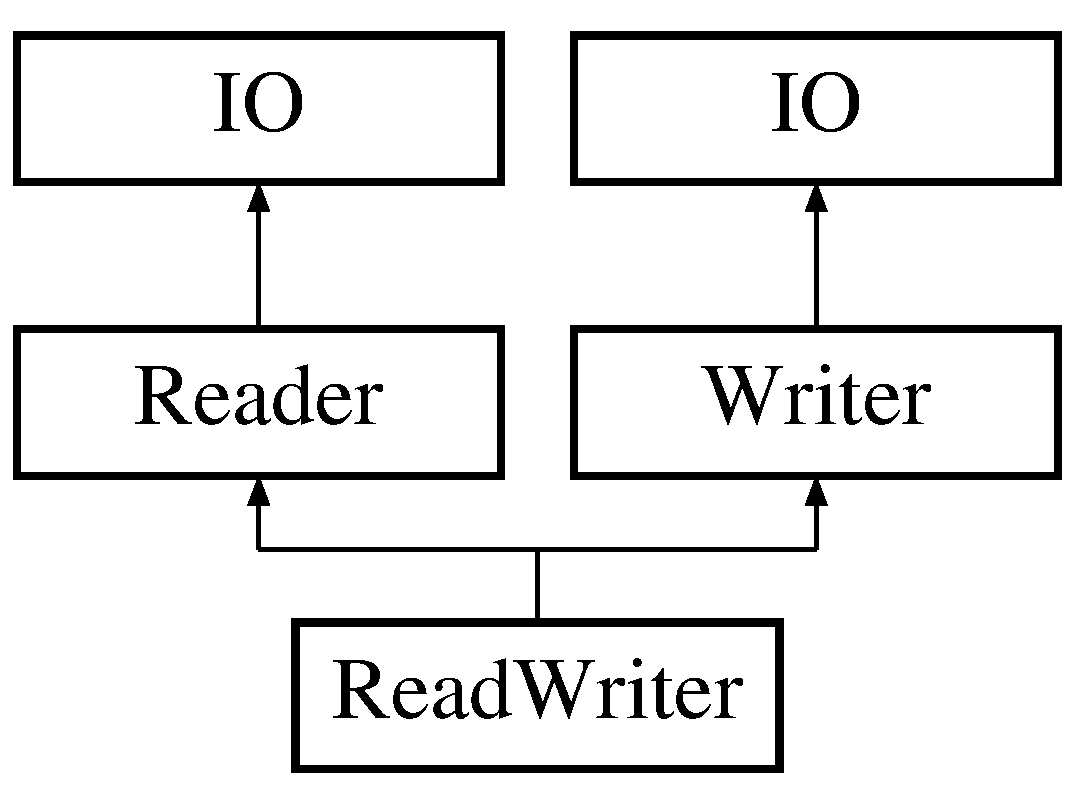
\includegraphics[height=3.000000cm]{class_read_writer}
\end{center}
\end{figure}
\subsection*{Public Member Functions}
\begin{DoxyCompactItemize}
\item 
\mbox{\Hypertarget{class_read_writer_a0321fa44af6d2da78daa62bb9ab4f7f9}\label{class_read_writer_a0321fa44af6d2da78daa62bb9ab4f7f9}} 
{\bfseries Read\+Writer} (string p=I\+O\+::get\+Default\+Path())
\end{DoxyCompactItemize}
\subsection*{Additional Inherited Members}


The documentation for this class was generated from the following file\+:\begin{DoxyCompactItemize}
\item 
Read\+Writer.\+h\end{DoxyCompactItemize}

\hypertarget{struct_register}{}\section{Register Struct Reference}
\label{struct_register}\index{Register@{Register}}
\subsection*{Public Member Functions}
\begin{DoxyCompactItemize}
\item 
\mbox{\Hypertarget{struct_register_ae4aeeaaefcbac30c5fc69df508afcabb}\label{struct_register_ae4aeeaaefcbac30c5fc69df508afcabb}} 
{\bfseries Register} (string name, \hyperlink{class_adj}{Adj} $\ast$($\ast$func)())
\end{DoxyCompactItemize}
\subsection*{Public Attributes}
\begin{DoxyCompactItemize}
\item 
\mbox{\Hypertarget{struct_register_a590c76fe1eaf40599a1ebf808249cb4d}\label{struct_register_a590c76fe1eaf40599a1ebf808249cb4d}} 
string {\bfseries keyword}
\end{DoxyCompactItemize}


The documentation for this struct was generated from the following file\+:\begin{DoxyCompactItemize}
\item 
Register.\+h\end{DoxyCompactItemize}

\hypertarget{class_writer}{}\section{Writer Class Reference}
\label{class_writer}\index{Writer@{Writer}}
Inheritance diagram for Writer\+:\begin{figure}[H]
\begin{center}
\leavevmode
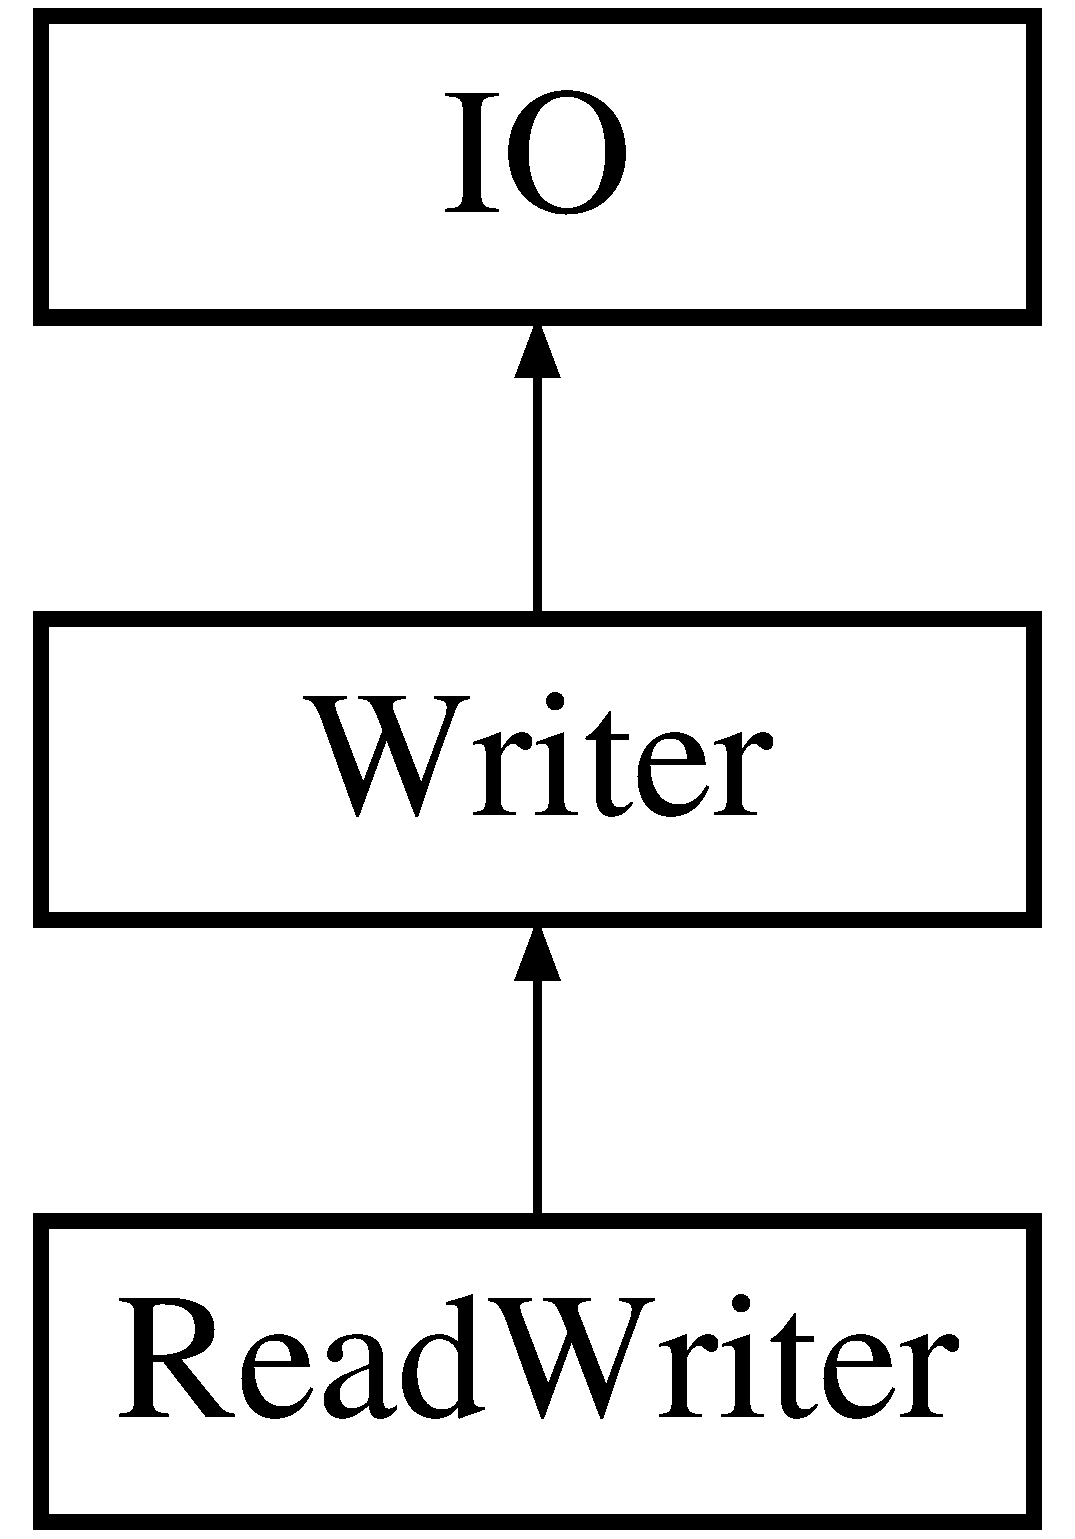
\includegraphics[height=3.000000cm]{class_writer}
\end{center}
\end{figure}
\subsection*{Public Member Functions}
\begin{DoxyCompactItemize}
\item 
\mbox{\Hypertarget{class_writer_a1754ec3741573fef15043d5e4b29f14f}\label{class_writer_a1754ec3741573fef15043d5e4b29f14f}} 
{\bfseries Writer} (string p=I\+O\+::get\+Default\+Path())
\item 
\mbox{\Hypertarget{class_writer_a285f9a71846bc81fe7de2575c72db480}\label{class_writer_a285f9a71846bc81fe7de2575c72db480}} 
{\footnotesize template$<$typename R , typename T $>$ }\\void {\bfseries write\+File} (\hyperlink{class_bio_net}{Bio\+Net}$<$ T $>$ \&bn, string \&fname, bool use\+Default=true)
\end{DoxyCompactItemize}
\subsection*{Additional Inherited Members}


The documentation for this class was generated from the following file\+:\begin{DoxyCompactItemize}
\item 
Writer.\+h\end{DoxyCompactItemize}

%--- End generated contents ---

% Index
\backmatter
\newpage
\phantomsection
\clearemptydoublepage
\addcontentsline{toc}{chapter}{Index}
\printindex

\end{document}
